%!TEX root = ../../ThesisRomainbrault.tex

%------------------------------------------------------------------------------
\section{Notations}
In this section we summarize briefly important notions used throughout this
document. It is mainly based on books and lecture notes of
\citet{kurdila2006convex,cotaescu2016elements}.

\subsection{Algebraic structures}
\label{sec:notations}
We note $\mathbb{K}$ any Abelian\mpar{Commutative.} field, $\mathbb{R}$ the
Abelian field of real numbers and $\mathbb{C}$ the Abelian field of complex
numbers. The unit pure imaginary number $\sqrt{-1}\in\mathbb{C}$ is denoted
$\iu$ and the Euler constant $\exp(1)\in\mathbb{R}$ is denoted $\ec$.
$\mathbb{N}$ represents the set of natural numbers and $\mathbb{N}_n$,
$n\in\mathbb{N}$ the set of natural numbers smaller or equal to $n$. For any
space $\mathcal{S}$, $\mathcal{S}^d$, $d\in\mathbb{N}$ represents the Cartesian
product space $\mathcal{S}^d = \mathcal{S}\times\cdots\times\mathcal{S}$. For
any two algebraic structures $\mathcal{S}$ and $\mathcal{S}'$ we write
$\mathcal{S}\cong\mathcal{S}'$ is there exist an isomorphism between these two
structures. If $a+\iu b = x \in \mathbb{C}$ then $\conj{x}=a-\iu
b\in\mathbb{C}$ denote the complex conjugate. By extension if $x\in\mathbb{R}$,
$\conj{x}=x\in\mathbb{R}$.

\subsection{Topology and continuity}
In order to define a proper notion of continuity, we focus on topological
spaces. A topological space is a pair of sets $(\mathcal{X},\mathcal{T}_x)$
where $\mathcal{X}$ describes the points considered, and $\mathcal{T}_x$
describes the possible neighbourhoods. The standards axioms of topology suppose
that $\mathcal{T}_x\subseteq{\mathcal{P}(\mathcal{X})}$ is a collection of
subsets of $\mathcal{X}$ such that the empty set and $\mathcal{X}$ itself
belongs to $\mathcal{T}_x$, any (finite or infinite) union of members of
$\mathcal{T}_x$ still belongs to $\mathcal{T}_x$ and the intersection of any
finite number of members of $\mathcal{T}_x$ still belongs to $\mathcal{T}_x$.
The elements of $\mathcal{T}_x$ are called open sets and the collection
$\mathcal{T}_x$ is a topology on $\mathcal{X}$. If
$(\mathcal{X},\mathcal{T}_x)$ and $(\mathcal{Y},\mathcal{T}_y)$ are topological
spaces, a function $f$ is said to be continuous if for every open set
$\mathcal{V}\in \mathcal{T}_y$, the inverse image $f^{-1}(\mathcal{V}) = \Set{
x \in \mathcal{X} | f ( x ) \in \mathcal{V} }$ is an open subset of
$\mathcal{T}_x$. Since the notion of continuity depends on open sets, it
depends on the topology of the spaces $\mathcal{X}$ and $\mathcal{Y}$.
\paragraph{}
If $\mathcal{X}$ is a topological space and $x$ is a point in $\mathcal{X}$, a
neighbourhood of $x$ is a subset $\mathcal{V}$ of $\mathcal{X}$ that includes
an \emph{open} set $\mathcal{U}$ containing $x$. A topological space
$\mathcal{X}$ is said to be Hausdorff (T2) when all distinct points in
$\mathcal{X}$ are pairwise neighborhood-separable. \acs{ie}~if there exists a
neighbourhood $\mathcal{U}$ of $x$ and a neighbourhood $\mathcal{V}$ of $y$
such that $\mathcal{U}$ and $\mathcal{V}$ are disjoint. It implies the
uniqueness of limits of sequences and existence of nets used throughout this
thesis. Therefore in the whole document we always assume that a topological
space $\mathcal{X}$ is Haussdorff.
\paragraph{}
A topological space is said to be second countable if it has a countable base.
Every second-countable space is separable and Lindel\"of\mpar{Every open cover
has a countable subcover.} (The reverse implications do not hold). A space is
metrisable if and only if it is second countable.
\paragraph{}
A topological space is said to be separable if there exists a sequence
$(x_n)_{n\in\mathbb{N}^*}$ of elements of $\mathcal{X}$ such that every
nonempty open subsets of the space contains at least one element of the
sequence. Separability plays an important role in numerical analysis because
many theorems have only constructive proofs for separable spaces. Such
constructive proofs can be turned into algorithms which is the primary goal of
this work. In this document we also assume that any topological space is
separable if there is no specific mention of the contrary. Moreover we recall
that a Hilbert space is separable if and only if it has a countable orthonormal
basis (Hence separable Hilbert spaces are second countable). Hence an operator
between two separable Hilbert spaces can be written as an infinite dimensional
matrix. In some cases we also introduce \emph{Polish spaces} which are
separable topological spaces $\mathcal{X}$ that pocess at least one $d$ metric
such that $(\mathcal{X}, d)$ is complete. Then $d$ induces the topology
$\mathcal{T}_x$ of $\mathcal{X}$. As metrisable spaces, Polish spaces are always
second countable. Moreover ervery second countable locally compact Hausdorff
space is a Polish space and every separable Banach space is a Polish space.
\paragraph{}
If $\mathcal{X}$ and $\mathcal{Y}$ are two topological spaces, we denote by
$\mathcal{F}(\mathcal{X};\mathcal{Y})$ the topological vector space of
functions $f:\mathcal{X}\to\mathcal{Y}$ and
$\mathcal{C}(\mathcal{X};\mathcal{Y}) \subset
\mathcal{F}(\mathcal{X};\mathcal{Y})$ the subspace of continuous functions,
endowed with the product topology (topology of pointwise convergence).

\subsection{Measure theory}
A $\sigma$-algebra on $\mathcal{X}$ is a set
$\mathcal{M}\subseteq\mathcal{P}(\mathcal{X})$ of subsets of $\mathcal{X}$,
containing the empty set, which is closed under taking complements and
countable unions. A pair $(\mathcal{X},\mathcal{M})$ where $\mathcal{X}$ is a
set and $\mathcal{M}$ is a $\sigma$-algebra is called a measure space. The
Borel $\sigma$-algebra $\mathcal{B}(\mathcal{X})$ is a $\sigma$-algebra
generated by the open sets of $\mathcal{X}$. A measure on a measurable space
$(\mathcal{X},\mathcal{B}(\mathcal{X}))$ is a map $\mu: \mathcal{B}(X) \to
\overline{\mathbb{R}}_+$ which is zero on the empty set and countably additive,
\acs{ie}~for any subset $(\mathcal{Z}_n)_{n\in\mathbb{N}}$ is a sequence of
pairwise disjoint measurable sets, 
\begin{dmath*}
    \mu\left(\bigcup_{n\in\mathbb{N}}\mathcal{Z}_n\right) =
    \sum_{n\in\mathbb{N}}\mu(\mathcal{Z}_n).
\end{dmath*}

\subsection{Vector spaces, linear operators and matrices}
Given any vector space $\mathcal{H}$ over an Abelian field $\mathbb{K}$, the
(continuous) dual space\footnote{The continuous dual space is also called
topological dual space. This must be differentiate from the \emph{algebraic}
dual space, which is the space of linear functionals from the original
vector-space to its base field. Hence the continuous dual space is a subset of
the algebraic dual space. The continuous and the algebraic dual space only
match when considering finite dimensional vector-spaces} $\mathcal{H}^\adjoint$
is defined as the set of all \emph{continuous} linear functionals $x^*:
\mathcal{H} \to \mathbb{K}$. When $\mathcal{H}$ is a vector space, there is a
natural duality pairing between $\mathcal{H}^\adjoint$ and $\mathcal{H}$
defined for all $x^\adjoint\in\mathcal{H}^\adjoint$ and all $z\in\mathcal{H}$
as $\pairing{x^\adjoint, z}_{\mathcal{H}^\adjoint, \mathcal{H}} = x^\adjoint(z)
= x^\adjoint z$. The duality paring $\pairing{\cdot,
\cdot}_{\mathcal{H}^\adjoint,\mathcal{H}}$ is then a bilinear form.
\paragraph{}
Let $\mathcal{H}_1$ and $\mathcal{H}_2$ be two vector spaces.  We call operator
any linear function from $\mathcal{H}_1$ to $\mathcal{H}_2$ The transpose (or
dual) of an operator $W:~\mathcal{H}_1\to\mathcal{H}_2$ is defined as
$W^\transpose :\mathcal{H}_2^\adjoint \to \mathcal{H}_1^\adjoint$ such that
$W^\transpose :x^\adjoint\mapsto x^\adjoint(W)$. It is characterized by the
relation $\pairing*{x^\adjoint,
Wz}_{\mathcal{H}_2^\adjoint,\mathcal{H}_2}=\pairing*{W^\transpose x^\adjoint,
z}_{\mathcal{H}_1^\adjoint,\mathcal{H}_1}$ for all
$x^\adjoint\in\mathcal{H}_2^\adjoint$ and all $z\in\mathcal{H}_1$. An operator
is called self-dual when $W^\transpose =W$.
\paragraph{}
Let $\mathcal{H}_1$ and $\mathcal{H_2}$ be two vector space. We set
$\mathcal{L}(\mathcal{H}_1;\mathcal{H}_2)$ to be the space of \emph{bounded}
(linear) operators from $\mathcal{H}_1$ to $\mathcal{H}_2$. The vector space
$\mathcal{H}_1$ is called the domain, noted $\Dom$ and $\mathcal{H}_2$ the
codomain. We use the shortcut notation
$\mathcal{L}(\mathcal{H})=\mathcal{L}(\mathcal{H}, \mathcal{H})$.
Interestingly if $\mathcal{H}_1$ and $\mathcal{H}_2$ are normed vector spaces,
they can be viewed as topological vector spaces, and the notion of continuity
coincides with that of boundedness. We recall the the norm of a linear operator
is given by
\begin{dmath*}
    \norm{W}_{\mathcal{H_1},\mathcal{H}_2} = \sup_{x\neq 0}
    \frac{\norm{W x}_{\mathcal{H}_2}}{\norm{x}_{\mathcal{H}_1}}.
\end{dmath*}
If $W\in\mathcal{L}(\mathcal{H}_1, \mathcal{H}_2)$
\begin{dmath*}
    \Ker W=\Set{x\in\Dom(W) | W x = 0}
\end{dmath*}
denotes the kernel (nullspace), which is a vector subspace of the domain and
\begin{dmath*}
    \Ima W = \Set{y\in\mathcal{H}_2 | y =Wx,\enskip x \in \Dom(W)}
\end{dmath*}
the image (range) which is a vector subspace of the codomain $\mathcal{H}_2$.
\paragraph{}
If $\mathcal{H}$ is an Hilbert space on a field $\mathbb{K}$ we denote its
scalar product by $\inner{\cdot,\cdot}_{\mathcal{H}}$ and its norm by
$\norm{\cdot}_{\mathcal{H}}$. When the base field of $\mathcal{H}$ is
$\mathbb{R}$, $\inner{\cdot,\cdot}_{\mathcal{H}}$ is a \emph{bilinear} form.
When the base field of $\mathcal{H}$ is $\mathbb{C}$,
$\inner{\cdot,\cdot}_{\mathcal{H}}$ is a \emph{sesquilinear} form.
\paragraph{}
Let $\mathcal{H}$ be a Hilbert space. From Riesz's representation theorem,
there is a unique isometric isomorphism
$\iota_R:\mathcal{H}\to\mathcal{H}^\adjoint$ such that for any $x$ and
$y\in\mathcal{H}$, $\pairing{\iota_R(x), y}_{\mathcal{H}^\adjoint,
\mathcal{H}}=\inner{x,y}_{\mathcal{H}}$ and
$\norm{\iota_R(x)}_{\mathcal{H}^\adjoint}=\norm{x}_{\mathcal{H}}$. The Riesz
map $\iota_R$ is self-dual, thus if $\mathcal{H}$ is a Hilbert space,
$\mathcal{H}$ is reflexive.
\acs{ie}~$\mathcal{H}^{\adjoint\adjoint}\cong\mathcal{H}$. When the base field
of $\mathcal{H}$ is $\mathbb{C}$, then $\iota_R$ is an \emph{anti-linear} form
since $\inner{\cdot,\cdot}_{\mathcal{H}}$ is sesquilinear and $\pairing{\cdot,
\cdot}_{\mathcal{H}^\adjoint, \mathcal{H}}$ is bilinear. In the same way when
the base field of $\mathcal{H}$ is $\mathbb{R}$ then $\iota_R$ is \emph{linear}
since both $\inner{\cdot,\cdot}_{\mathcal{H}}$ and $\pairing{\cdot,
\cdot}_{\mathcal{H}^\adjoint, \mathcal{H}}$ are bilinear. If $\mathcal{H}$ is a
Hilbert space we make the dual space $\mathcal{H}^\adjoint$ a Hilbert space by
endowing it with the inner product $\inner{x^\adjoint,
z^\adjoint}_{\mathcal{H}^\adjoint}=\inner{\iota_R^{-1}(x^\adjoint),
\iota_R^{-1}(z^\adjoint)}_{\mathcal{H}}$ for all $x^\adjoint$,
$z^\adjoint\in\mathcal{H}^\adjoint$.
\paragraph{}
Let $\mathcal{H}_1$ and $\mathcal{H}_2$ be two Hilbert spaces. The adjoint of
an operator $W:\mathcal{H}_1\to\mathcal{H}_2$ is the unique mapping
$W^\adjoint:\mathcal{H}_2\to\mathcal{H}_1$ such that $\inner{W^\adjoint x,
z}_{\mathcal{H}_1}=\inner{x, Wz}_{\mathcal{H}_2}$ for all
$x\in\Dom(W^\adjoint)$, $z\in\Dom(W)$. Its existence is guaranteed by Riesz's
representation theorem. An operator
$W:\Dom(W)\subseteq\mathcal{H}\to\mathcal{H}$ is said to be symmetric when
$W^\adjoint=W$ and self-adjoint when $W$ is bounded, symmetric,
$\Dom(W^\adjoint) = \Dom(W)$ and $\Dom(W)$ is dense in $\mathcal{H}$. If $W$
is bounded, symmetric and $\Dom(W)=\mathcal{H}$ then $W$ is self-adjoint.
Notice that the transpose is linked to the adjoint by the relation $W^\adjoint
= \iota_R^{-1} W^\transpose \iota_R$. When $\mathcal{H}$ is a Hilbert space, if
$x\in\mathcal{H}$, we always define $x^\adjoint\in\mathcal{H}^\adjoint$ to be
\begin{dmath*}
    x^\adjoint\hiderel{=}\iota_R(x)\hiderel{=}\inner{x, \cdot}_{\mathcal{H}}.
\end{dmath*}
\begin{figure}[htb]
    \centering
    \begin{tikzcd}[matrix scale=3]
            \mathcal{H}_2 \arrow[r, "W^\adjoint"] \arrow[d, "\iota_R"] &
            \mathcal{H}_1  \arrow[d, bend left, "\iota_R"] \\
            \mathcal{H}_2^\adjoint  \arrow[r, "W^\transpose "] &
            \mathcal{H}_1^\adjoint \arrow[u, bend left, "\iota_R^{-1}"]
    \end{tikzcd}
    \caption{\label{fig:riesz_map}Riesz map, dual spaces and adjoints.}
\end{figure}
\paragraph{}
Let $\mathcal{H}$ be a \emph{separable} Hilbert space and let
$(e_i)_{i\in\mathbb{N}^*}$ be a basis of $\mathcal{H}$. We call
$(e_i^\adjoint)_{i\in\mathbb{N}^*}$ the dual basis of $\mathcal{H}$, the basis
of $\mathcal{H}^\adjoint$ such that for all $i$, $j\in\mathbb{N}^*$,
$e_i^\adjoint(e_j)=\inner{e_i, e_j}_{\mathcal{H}}=\delta_{ij}$. In the whole
document we consider that $\mathcal{H}^\adjoint$ is always equipped with the
dual basis of $\mathcal{H}$.  For a vector $x\in\mathcal{H}$ with a basis
$(e_i)_{i\in\mathbb{N}^*}$ we write $x_i=e_i^\adjoint(x)$. For a linear
operator $W:\mathcal{H}_1\to\mathcal{H}_2$ where $\mathcal{H}_1$ and
$\mathcal{H}_2$ are Hilbert spaces with respective basis
$(e_i)_{i\in\mathbb{N}^*}$ and $(e'_j)_{j\in\mathbb{N}^*}$, we note $W_i=We_i$
and $W_{ij}=e_j^\adjoint(We_i)$. Eventually given two separable Hilbert spaces
$\mathcal{H}_1$ and $\mathcal{H}_2$, an operator
$W:\mathcal{H}_1\to\mathcal{H}_2$, $(e_i)_{i\in\mathbb{N}^*}$ a basis of
$\mathcal{H}_1$ and $(e'_i)_{i\in\mathbb{N}^*}$ a basis of $\mathcal{H}_2$ we
have
\begin{dmath*}
    (W^\transpose)_{ij}=e_j^{\adjoint\adjoint}W^\transpose
    {e'}_i^\adjoint\hiderel{=} e_j^{\adjoint\adjoint}{e'}_i^\adjoint W
    \hiderel{=} {e'}_i^\adjoint W e_j \hiderel{=} W_{ji}.
\end{dmath*}
\paragraph{}
We call matrix $M$ of size $(m,n)\in\mathbb{N}^2$ on an Abelian field
$\mathbb{K}$ a collection of elements $M=(m_{ij})_{1\le i\le m, 1\le j \le n}$,
$m_{ij}\in\mathbb{K}$. We note $\mathcal{M}_{m,n}(\mathbb{K})$ the vector space
of all matrices. If $\mathcal{H}_1$ and $\mathcal{H}_2$ are two separable
Hilbert spaces on an Abelian field $\mathbb{K}$, any linear operator
$L\in\mathcal{L}(\mathcal{H}_1;\mathcal{H}_2)$ can be viewed as a (potentially
infinite) matrix. Let $n=\dim(\mathcal{H}_1)$, $m=\dim(\mathcal{H}_2)$ and let
$B=(e_i)_{i=1}^{n}$ and $C=(e'_i)_{i=1}^{m}$ be the respective bases of
$\mathcal{H}_1$ and $\mathcal{H}_2$. We note $\text{mat}_{B, C}:
\mathcal{L}(\mathcal{H}_1;\mathcal{H}_2) \to \mathcal{M}_{m,n}(\mathbb{K})$
such that $M=\text{mat}_{B, C}(L)=({e'}_j^\adjoint L e_i)_{1\le i\le n, 1\le j
\le m}\in\mathcal{M}_{m,n}(\mathbb{K})$. Let
$M_1\in\mathcal{M}_{m,n}(\mathbb{K})$ and
$M_2\in\mathcal{M}_{n,l}(\mathbb{K})$. The product between two matrices is
written $M_1M_2\in\mathcal{M}_{m,l}(\mathbb{K})$ and obey $(M_1M_2)_{ij} =
\sum_{k=1}^n M_{ik}M_{kj}$. Given two linear operator
$L_1\in\mathcal{L}(\mathcal{H}_1;\mathcal{H}_2)$ and
$L2\in\mathcal{L}(\mathcal{H}_2;\mathcal{H}_3)$ we have
$L_1L_2\in\mathcal{L}(\mathcal{H}_1;\mathcal{H}_3)$ and i
\begin{dmath*}
    \text{mat}_{B, D}(L_1L_2)=\text{mat}_{B, C}(L_1)\text{mat}_{C, D}(L_2).
\end{dmath*}
The operator $\text{mat}_{B, C}$ is a vector space isomorphism allowing us to
identify $\mathcal{L}(\mathcal{H}_1;\mathcal{H}_2)$ with
$\mathcal{M}_{mn}(\mathbb{K})$ where $n=\dim(\mathcal{H}_1)$ and
$m=\dim(\mathcal{H}_2)$. All these notations are summarized in
\cref{table:notations1,table:notations2}.
\begin{table}
    \centering
    \caption{Mathematical symbols used throughout the parper and their
    signification (part 1). \label{table:notations1}}
    \begin{tabularx}{\textwidth}{cX}
        \toprule
            Symbol & \multicolumn{1}{c}{Meaning} \\
        \cmidrule{1-2}
        \endhead
            $\colonequals$ & Equal by definition. \\
            $\mathbb{N}$ & The semi-group of natural numbers. \\
            $\mathbb{K}$ & Any non-discrete Abelian field endowed with an
            absolute value. Elements of $\mathbb{K}$ are called scalars. \\
            $\mathbb{R}$ & The Abelian field of real numbers. \\
            $\mathbb{C}$ & The Abelian field of complex numbers. \\
            $\mathbb{U}$ & The circle group of complex numbers with unit
            module. \\
            $\iu \in\mathbb{C}$ & Unit pure imaginary number
            $\iu^2\colonequals-1$.  \\
            $\ec \in\mathbb{R}$ & Euler constant. \\
            $e \in \mathcal{X}$ &  The neutral element of the group
            $\mathcal{X}$. \\
            $\delta_{ij}$ & Kronecker delta function. $\delta_{ij}=0$ if $i
            \neq j$, $1$ otherwise. \\
            $\inner{\cdot,\cdot}_2$ & Euclidean inner product. \\
            $\norm{\cdot}_2$ & Euclidean norm. \\
            $\mathcal{X}$ & Input space. \\
            $\dual{\mathcal{X}}$ & The Pontryagin dual of $\mathcal{X}$ when
            $\mathcal{X}$ is a \acs{LCA} group. \\
            $\mathcal{Y}$ & Output space (Hilbert space). \\
            $\mathcal{H}$ & Feature space (Hilbert space).  \\ 
            $\inner{\cdot,\cdot}_{\mathcal{Y}}$ & The canonical inner
            product of the Hilbert space $\mathcal{Y}$. \\
            $\norm{\cdot}_{\mathcal{Y}}$ & The canonical norm induced by the
            inner product of the Hilbert space $\mathcal{Y}$. \\
            $\mathcal{F}(\mathcal{X};\mathcal{Y})$ & Topological vector space
            of functions from $\mathcal{X}$ to $\mathcal{Y}$. \\
            $\mathcal{C}(\mathcal{X};\mathcal{Y})$ & The topological vector
            subspace of $\mathcal{F}$ of continuous functions from
            $\mathcal{X}$ to $\mathcal{Y}$. \\
            $\mathcal{L}(\mathcal{H};\mathcal{Y})$ & The set of bounded linear
            operator from a Hilbert space $\mathcal{H}$ to a
            Hilbert space $\mathcal{Y}$. \\
            $\norm{\cdot}_{\mathcal{Y},\mathcal{Y}'}$ & The operator norm
            $\norm{\Gamma}_{\mathcal{Y}, \mathcal{Y'}} =
            \sup_{\norm{y}_{\mathcal{Y}}=1}\norm{\Gamma y}_{\mathcal{Y}'}$ for
            all $\Gamma\in\mathcal{L}(\mathcal{Y},\mathcal{Y'})$ \\
            $\mathcal{M}_{m,n}(\mathbb{K})$ & The set of matrices of size
            $(m,n)$. \\
            $\mathcal{L}(\mathcal{Y})$ & The set of bounded linear operator
            from a Hilbert space $\mathcal{Y}$ to itself. \\
            $\mathcal{L}_{+}(\mathcal{Y})$ & The set of non-negative bounded
            linear operator from a Hilbert space $\mathcal{H}$ to itself. \\
            $\mathcal{B}(\mathcal{X})$ & Borel $\sigma$-algebra on a
            topological space $\mathcal{X}$. \\
            $\mu(\mathcal{X})$ & A scalar positive measure of $\mathcal{X}$. \\
            $\Leb(\mathcal{X})$ & The Lebesgue measure of $\mathcal{X}$. \\
            $\Haar(\mathcal{X})$ & A Haar measure of $\mathcal{X}$. \\
        \bottomrule
    \end{tabularx}
\end{table}
\begin{table}
    \centering
    \caption{Mathematical symbols used throughout the parper and their
    signification (part 2). \label{table:notations2}}
    \begin{tabularx}{\textwidth}{cX}
        \toprule
            Symbol & \multicolumn{1}{c}{Meaning} \\
        \cmidrule{1-2}
        \endhead
            $\probability_{\mu, \rho}(\mathcal{X})$ & A probability measure of
            $\mathcal{X}$ whose Radon-Nikodym derivative with respect to the
            measure $\mu$ is $\rho$. \\
            $\FT{\cdot}$ & The \acl{FT} operator. \\
            $\IFT{\cdot}$ & The \acl{IFT} operator. \\
            $\esssup$ & The essential supremum. \\
            $L^p(\mathcal{X}, \mu)$ & The Banach space of
            $\abs{\cdot}^p$-integrable function from
            $(\mathcal{X},\mathcal{B}(\mathcal{X}), \mu)$ to $\mathbb{C}$ for
            $p\in\mathbb{R}_+$. \\
            $L^p(\mathcal{X}, \mu;\mathcal{Y})$ & The Banach space of
            $\norm{\cdot}_{\mathcal{Y}}^p$ (Bochner)-integrable function from
            $(\mathcal{X},\mathcal{B}(\mathcal{X}), \mu)$ to $\mathcal{Y}$ for
            $p\in\mathbb{R}_+$. $L^p(\mathcal{X},\mu,\mathbb{R}) \colonequals
            L^p(\mathcal{X},\mu)$. \\
            $\Vect_{j=1}^D x_i$ & The direct sum of $D\in\mathbb{N}$ vectors
            $x_i$'s in the Hilbert spaces $\mathcal{H}_i$. \\
            $\norm{\cdot}_p$ & The $L^p(\mathcal{X}, \mu, \mathcal{Y})$ norm.
            $\norm{f}_p^p\colonequals \int_{\mathcal{X}}
            \norm{f(x)}_{\mathcal{Y}}^p d\mu(x)$.  When
            $\mathcal{X}=\mathbb{N}^*$, $\mathcal{Y}\subseteq \mathbb{R}$ and
            $\mu$ is the counting measure and $p=2$ it co\"incide with the
            Euclidean norm $\norm{\cdot}_2$ for finite dimensional vectors. \\
            $\norm{\cdot}_{\infty}$ & The uniform norm $\norm{f}_{\infty}=
            \esssup \set{\norm{f(x)}_{\mathcal{Y}} |
            x\in\mathcal{X}}=\lim_{p\to\infty}\norm{f}_p$. \\
            ${}^\transpose$ & The transpose operator of a linear operator. \\
            ${}^\adjoint$ & The adjoint operator of a linear operator. \\
            $\abs{\Gamma}$ & The absolute value of the linear operator
            $\Gamma\in\mathcal{L}(\mathcal{Y})$, \acs{ie}
            $\abs{\Gamma}^2=\Gamma^{\adjoint}\Gamma$. \\
            $\Tr\left[\Gamma\right]$ & The trace of a linear operator
            $\Gamma\in\mathcal{L}(\mathcal{Y})$. \\
            $\sigma(\Gamma)$ & The spectrum of the bounded linear operator
            $Gamma\in\mathcal{L}(\mathcal{Y})$ where $\mathcal{Y}$ is a Hilbert
            space, \acs{ie}~$\sigma(\Gamma)=\Set{\lambda\in\mathbb{C} |
            \nexists s, s(\lambda e - \Gamma) = e}$. \\
            $\lambda_i(\Gamma)$ & The $i$-th eigenvalue of
            $\Gamma\in\mathcal{L}(\mathcal{Y})$, ranked by increasing modulus,
            where $\mathcal{Y}$ is a \emph{separable} Hilbert space and
            $i\in\mathbb{N}^*$. \\
            $\rho(\Gamma)$ & The spectral radius of the linear operator
            $\Gamma$ \acs{ie}~$\rho(\Gamma)=\sup\set{\abs{\lambda} | \lambda
            \in \sigma(\Gamma)}$. \\
            $\norm{\cdot}_{\sigma, p}$ & The Schatten $p$-norm,
            $\norm{\Gamma}_{\sigma,
            p}^p=\Tr\left[\abs{\Gamma}^p\right]$ for
            $\Gamma\in\mathcal{L}(\mathcal{Y})$, where $\mathcal{Y}$ is a
            Hilbert space. Note that $\norm{\Gamma}_{\sigma,\infty} =
            \rho(\Gamma) \le \norm{\Gamma}_{\mathcal{Y},\mathcal{Y}}$.  \\
            $\succcurlyeq$ & \say{Greater than} in the Loewner partial order of
            operators. $\Gamma_1 \succcurlyeq \Gamma_2$ if $\sigma(\Gamma_1 -
            \Gamma_2) \subseteq \mathbb{R}_+$. \\
            $\bar{\mathbb{R}}$ & The one point compacification of the real
            line $\mathbb{R} \cup \Set{\infty}$. \\
            $\cong$ & Given two sets $\mathcal{X}$ and $\mathcal{Y}$,
            $\mathcal{X} \cong \mathcal{Y}$ if there exists an isomorphism
            $\phi:\mathcal{X}\to\mathcal{Y}$. \\
        \bottomrule
    \end{tabularx}
\end{table}
% \FloatBarrier

%------------------------------------------------------------------------------
\section{About statistical learning}
\label{sec:about_statistical_learning}

%------------------------------------------------------------------------------
\section{On large-scale learning}
\label{sec:on_large-scale_learning}

\section{History and state of the art of large scale learning with kernels}
\label{sec:history}

\subsection{Introduction to kernel methods}



\subsection{Quadratic programing, subsampling}

\subsection{Gradient descents}

\subsection{Mercer Theorem, Nystr\"om method and feature maps}
\subsubsection{Nystr\"om approximations}
To overcome the bottleneck of Gram matrix computations in kernel methods,
Williams and Seeger \cite{Williams2000-nystrom} have proposed to generate a
low-rank matrix approximation of the Gram matrix using a subset of its columns.
\subsubsection{Random Fourier Feature maps}
Random Fourier Feature methodology introduced  by Rahimi and Recht
\cite{Rahimi2007} provides a way to scale up kernel methods when kernels are
Mercer and \emph{translation-invariant}  for the group law considered on the
input space $\mathcal{X}$. We describe here the original approach proposed in
\cite{Rahimi2007}, focusing on the group $(\mathbb{R}^d, +)$. Extensions to
other group laws such as \cite{li2010random} are described in
\cref{subsubsec:skewedchi2} within the general framework of operator-valued
kernels.
\paragraph{}
Denote $k: \mathbb{R}^d \times \mathbb{R}^d \to \mathbb{R}$ a positive
definite kernel on $\mathbb{R}^d$. A kernel $k$ is said to be
\emph{shift-invariant} or \emph{translation-invariant} for the addition if for
any $a \in \mathbb{R}^d$, and for all $(x,x') \in \mathbb{R}^d \times
\mathbb{R}^d$ we have $k(x+a,z+a) = k(x,z)$.  Then, we define $k_0: \mathbb{R}^d
\to \mathbb{R}$ the function such that $k(x,z)= k_0(x-z)$. $k_0$ is
called the \emph{signature} of kernel $k$. Bochner's theorem
\cite{folland1994course} is the theoretical result that leads to the Random
Fourier Features.
\begin{theorem}[Bochner's theorem]\label{th:bochner-scalar}
    Any continuous positive definite complex function is the \acl{FT} of a
    non-negative measure.
\end{theorem}
It implies that any positive definite, continuous and shift-invariant kernel
$k$, have a continuous and positive definite signature $k_0$, which is the
\acl{FT} of a non-negative measure $\mu$. We therefore have the following
corollary.
\begin{corollary}\label{c:bochner-app}
    With the previous notations and assumptions on $k$,
    \begin{dmath}\label{bochner-scalar}
        k(x,z)=k_0(x-z) = \int_{\mathbb{R}^d} e^{-\iu \inner{\omega,x - z}}
        d\mu(\omega).
    \end{dmath}
\end{corollary}
Without loss of generality, we assume that $\mu$ is a probability measure,
\acs{ie} $\int_{\mathbb{R}^d} d\mu(\omega)=1$ by renormalising the kernel since
\begin{dmath*}
    \int_{\mathbb{R}^d}d\mu(\omega)= \int_{\mathbb{R}^d}e^{-\iu \inner{\omega,
    0}d\mu(\omega)}=k_0(0). 
\end{dmath*}
Then we can write \cref{bochner-scalar} as an
expectation over $\mu$. For all $x$,
$z\in\mathbb{R}^d$
\begin{dmath*}
    k_0(x-z) = \expectation_{\mu}\left[e^{-\iu \inner{\omega,x - z}}\right].
\end{dmath*}
Eventuallt, if $k$ is real valued we only write the real part, $k(x,z)$ =
$\expectation_{\mu}[\cos \inner{\omega,x - z}]$ =$\expectation_{\mu}[ \cos
\inner{\omega,z}$ $\cos \inner{\omega,x}$ + $\sin \inner{\omega,z}$ $\sin
\inner{\omega,x}]$.  Let $\Vect_{j=1}^D x_j$ denote the $Dm$-length column
vector obtained by stacking vectors $x_j \in \mathbb{R}^m$.  The feature map
$\tilde{\phi}: \mathbb{R}^d \rightarrow \mathbb{R}^{2D}$ defined as
\begin{dmath}
\label{eq:rff}
    \tilde{\phi}(x)=\frac{1}{\sqrt{D}}\Vect_{j=1}^D
    \begin{pmatrix} 
        \cos{\inner{x,\omega_j}} \\
        \sin{\inner{x,\omega_j}}
    \end{pmatrix}, \enskip \omega_j \hiderel{\sim} \mu
\end{dmath}
is called a \emph{Random Fourier Feature} (map). Each $\omega_{j}, j=1, \ldots,
D$ is independently and identically sampled from the inverse Fourier transform
$\mu$ of $k_0$.  This Random Fourier Feature map provides the following
Monte-Carlo estimator of the kernel: $\tilde{k}(x, z) = \tilde{\phi}(x)^*
\tilde{\phi}(z)$. 
\paragraph{}
The dimension $D$ governs the precision of this
approximation, whose uniform convergence towards the target kernel (as defined
in \cref{bochner-scalar}) can be found in \citet{Rahimi2007} and in more recent
papers with some refinements proposed in \citet{sutherland2015} and
\citet{sriper2015}.  Finally, it is important to notice that Random Fourier
Feature approach \emph{only} requires two steps before the application of a
learning algorithm: (1) define the inverse Fourier transform of the given
shift-invariant kernel, (2) compute the randomized feature map using the
spectral distribution $\mu$.  \citet{Rahimi2007} show that for the Gaussian
kernel $k_0(x-z) = exp(-\gamma \norm{x - z}_2^2)$, the spectral distribution
$\mu(\omega)$ is a Gaussian distribution. For the Laplacian kernel $k_0(x-z) =
exp(-\gamma \norm{x - z}_1)$, the spectral distribution is a Cauchy
distribution.
\subsection{Recent extensions}

%------------------------------------------------------------------------------
\section{Elements of abstract harmonic analysis}
\label{sec:abstract_harmonic}

\subsection{Locally compact Abelian groups}
\begin{definition}[\acf{LCA} group.]
    A group $\mathcal{X}$ endowed with a binary operation $\groupop$ is said to
    be a Locally Compact Abelian group if $\mathcal{X}$ is a topological
    \emph{commutative} group \acs{wrt}~$\groupop$ for which every point has a
    compact neighborhood and is Hausdorff (T2).
\end{definition}
Moreover given a element $z$ of a \ac{LCA} group $\mathcal{X}$, we define the
set $z\groupop\mathcal{X}=\mathcal{X}\groupop z=\Set{z\groupop x|\forall
x\in\mathcal{X}}$ and the set $\mathcal{X}^{-1}=\Set{x^{-1}|\forall
x\in\mathcal{X}}$.  We also note $e$ the neutral element of $\mathcal{X}$ such
that $x\groupop e=e \groupop x= e$ for all $x\in\mathcal{X}$.  Throughout this
thesis we focus on positive definite function. Let $\mathcal{Y}$ be a complex
separable Hilbert space. A function $f:\mathcal{X}\to\mathcal{Y}$ is positive
definite if for all $N\in\mathbb{N}$ and all $y\in\mathcal{Y}$,
\begin{dmath}
    \label{eq:positive_definite} \sum_{i,j=1}^N\inner*{y_i,
    f\left(x_j^{-1}\groupop x_i\right)y_j}_{\mathcal{Y}}\ge 0
\end{dmath}
for all sequences $(y_i)_{i\in\mathbb{N}_N^*}\in\mathcal{Y}^N$ and all sequences
$(x_i)_{i\in\mathbb{N}_N^*}\in\mathcal{X}^N$. If $\mathcal{Y}$ is real we add
the assumption that $f(x^{-1})=f(x)^*$ for all $x\in\mathcal{X}$.  A
consequence is that a positive definite function is bounded, as shown by
\citet{falb1969theorem}, $\norm{f(x)}_{\mathcal{Y},\mathcal{Y}}\le
2\norm{f(e)}_{\mathcal{Y},\mathcal{Y}}$ for all $x\in\mathcal{X}$, however
positive definite functions are not necessarily continuous. This motivates the
introduction of functions of positive type which are nothing but continuous
positive definite function.

\subsection{The Haar measure}
Measures on topological spaces which appear in practice often satisfy the
following regularity properties.
\begin{definition}[Radon measure]
    A Radon measure $\mu=\Radon$ on a topological measurable space
    $\mathcal{X}$ is a measure on $(\mathcal{X}, \mathcal{B}(\mathcal{X}))$
    which satisfies the following properties.
    \begin{propenum}
        \item The measure $\Radon$ is finite on every compact set.
        \begin{dmath*}
            \Radon(K) < \infty\condition{for any compact set
            $K\in\mathcal{B}(\mathcal{X})$.}
        \end{dmath*}
        \item The measure $\Radon$ is outer regular on any Borel sets $E$.
        \begin{dmath*}
            \Radon(E)=\inf \Set{\Radon(U) | E\subseteq U}\condition{for any
            open set $U$.}
        \end{dmath*}
        \item The measure $\Radon$ is inner regular on open sets $E$.
        \begin{dmath*}
            \Radon(E)=\sup\Set{\Radon(K) | K\subseteq E}\condition{for any
            compact set $K$.}
        \end{dmath*}
    \end{propenum}
\end{definition}
When dealing with topological groups it is natural to look for measures which
are invariant under translation. There exist, up to a positive multiplicative
constant, a unique countably additive, nontrivial measure $\Haar$ on \emph{any}
$\ac{LCA}$ group. For more details and constructive proofs
see~\citet{alfsen1964simplified,folland1994course,conway2013course}.

\begin{definition}[The Haar measure]
    A Haar measure $\mu=\Haar$ on a \ac{LCA} group $\mathcal{X}=(G,\groupop)$
    is a Radon measure on $(\mathcal{X},\mathcal{B}(X))$ which is non-zero on
    non-empty open sets and is invariant under translation. Namely
    \begin{propenum}
        \item if $\mathcal{Z} \subseteq \mathcal{X}$ is open, then
        $\Haar(\mathcal{X})>0$.
        \item For all $\mathcal{Z}\in\mathcal{B}(\mathcal{X})$ and $x \in
        \mathcal{X}$, $\Haar(x\groupop \mathcal{Z})=\Haar(\mathcal{Z})$.
    \end{propenum}
\end{definition}
Such a measure on a \ac{LCA} group $\mathcal{X}$ is called a Haar
measure\mpar{If $\mathcal{X}$ was not supposed to be Abelian, we should have
defined a left Haar measure and a right Haar measure. In our case both measure
are the same, so we refer to both of them as Haar measure}. An immediate
consequence of the invariance is that for any $s\in\mathcal{X}$,
\begin{dmath*}
    \int_{\mathcal{X}}f(s\groupop x)d\Haar(x)=\int_{\mathcal{X}}f(x)d\Haar(x).
\end{dmath*}
It can be shown that $\Haar(U) > 0$ for every non-empty open subset $U$. In
particular, if $\mathcal{X}$ is compact then $\Haar(\mathcal{X})$ is finite and
positive, so we can uniquely specify a Haar measure on $\mathcal{X}$ by adding
the normalization condition $\Haar(\mathcal{X})=1$. We call measured space the
space $(\mathcal{X},\mathcal{B}(\mathcal{X}),\Haar)$ the space $\mathcal{X}$
endowed with its Borel $\sigma$-algebra and some measure $\Haar$. If
$\Haar(\mathcal{X})=1$ then the space
$(\mathcal{X},\mathcal{B}(\mathcal{X}),\Haar)$ is called a probability space.
Last but not least, on the additive group $(\mathbb{R},+)$, the Lebesgue
measure noted $\Leb$ is a valid Haar measure. For a concise introduction and
important properties we refer the reader to the lecture of
\citet{tornier2014haar}.

\subsection{Even and odd functions}
Let $\mathcal{X}$ be a \ac{LCA} group and $\mathbb{K}$ be a field viewed as an
additive group. We say that a function $f:\mathcal{X}\to\mathbb{K}$ is even if
for all $x\in\mathcal{X}$, $f(x)=f\left(\inv{x}\right)$ and odd if
$f(x)=-f\left(\inv{x}\right)$. The definition can be extended to
operator-valued functions.
\begin{definition}[Even and odd operator-valued function on a \ac{LCA} group]
    Let $\mathcal{X}$ be a measured \ac{LCA} group and $\mathcal{Y}$ be a
    Hilbert space, and $\mathcal{L}(\mathcal{Y})$ the space of bounded linear
    operators from $\mathcal{Y}$ to itself viewed as an additive group. A
    function $f:\mathcal{X}\to\mathcal{L}(\mathcal{Y})$ is (weakly) even if for
    all $x\in\mathcal{X}$ and all $y$, $y'\in\mathcal{Y}$,
    \begin{dmath}
        \inner{y,f\left(\inv{x}\right)y'}_{\mathcal{Y}} =
        \inner{y,f(x)y'}_{\mathcal{Y}}
    \end{dmath}
    and (weakly) odd if
    \begin{dmath}
        \inner{y,f\left(\inv{x}\right)y'}_{\mathcal{Y}} =
        -\inner{y,f(x)y'}_{\mathcal{Y}}
    \end{dmath}
\end{definition}
It is easy to check that if $f$ is odd then
$\int_{\mathcal{X}}\inner{y,f(x)y'}_{\mathcal{Y}}d\Haar(x)=0$.
\begin{proof}
    \begin{dmath*}
        \int_{\mathcal{X}} \inner{y, f(x)y'}_{\mathcal{Y}} d\Haar(x) =
        \int_{\mathcal{X}} \inner*{y, \left(\frac{f\left(\inv{x}\right)
        + f(x)}{2}\right)-\left(\frac{f\left(\inv{x}\right) -
        f(x)}{2}\right)y'}_{\mathcal{Y}}d\Haar(x)
        =\frac{1}{2} \left(-\int_{\mathcal{X}} \inner{y, f(x)y'}_{\mathcal{Y}}
        d\Haar(x) + \int_{\mathcal{X}}\inner{y,
        f(x)y'}_{\mathcal{Y}}d\Haar(x)\right)
        =0.
    \end{dmath*}
\end{proof}
Besides the product of an even and an odd function is odd. Indeed for all $f$,
$g\in\mathcal{F}(\mathcal{X};\mathcal{L}(\mathcal{Y}))$, where $f$ is even and
$g$ odd. Define $h(x)=\inner{y,f(x)g(x)y'}$. Then we have
\begin{dmath}
    h\left(\inv{x}\right) = \inner{y, f\left(\inv{x}\right)
    g\left(\inv{x}\right)y'}_{\mathcal{Y}}
    \hiderel{=}\inner{y,f(x)\left(-g(x)\right)y'}_{\mathcal{Y}}
    =-h(x).
\end{dmath}
\subsection{Characters}
\label{subsec:character} \acf{LCA} groups are central to the general definition
of Fourier Transform which is related to the concept of Pontryagin
duality~\citep{folland1994course}.  Let $(\mathcal{X}, \groupop)$ be a \ac{LCA}
group with $e$ its neutral element and the notation, $\inv{x}$, for the inverse
of $x \in \mathcal{X}$. A \emph{character} is a complex continuous homomorphism
$\omega:\mathcal{X}\to\mathbb{U}$ from $\mathcal{X}$ to the set of complex
numbers of unit module $\mathbb{U}$. The set of all characters of $\mathcal{X}$
forms the Pontryagin \emph{dual  group} $\dual{\mathcal{X}}$. The dual group of
an \ac{LCA} group is an \ac{LCA} group so that we can endow
$\dual{\mathcal{X}}$ with a \say{dual} Haar measure noted $\dual{\Haar}$. Then
the dual group operation is defined by
\begin{dmath*}
    (\omega_1 \groupop \omega_2)(x)=\omega_1(x)\omega_2(x) \hiderel{\in}
    \mathbb{U}.
\end{dmath*}
\paragraph{}
The Pontryagin duality theorem states that $\dual{\dual{\mathcal{X}}}\cong
\mathcal{X}$. \acs{ie}~there is a canonical isomorphism between any \ac{LCA}
group and its double dual. To emphasize this duality the following notation is
usually adopted
\begin{dmath}
    \label{eq:paringdef} \omega(x) = \pairing{x, \omega} \hiderel{=}
    \pairing{\omega, x} \hiderel{=} x(\omega),
\end{dmath}
where $x\in\mathcal{X}\cong\dual{\dual{\mathcal{X}}}$ and
$\omega\in\dual{\mathcal{X}}$. The form $\pairing{\cdot,\cdot}$ defined in
\cref{eq:paringdef} is called (duality) pairing. Another important property
involves the complex conjugate of the pairing which is defined as
\begin{dmath}
    \conj{\pairing{x, \omega}} = \pairing*{\inv{x}, \omega} \hiderel{=}
    \pairing*{x, \inv{\omega}}.
\end{dmath}
\begin{table}[htb]
    \caption{Classification of \acl{FT}s in terms of their domain and transform
    domain.}
    \label{tab:dual_and_pairing}
    \centering
    \begin{tabularx}{\textwidth}{cccX}
        \toprule
            \multicolumn{1}{c}{$\mathcal{X}=$} &
            \multicolumn{1}{c}{$\dual{\mathcal{X}}\cong$} &
            \multicolumn{1}{c}{Operation} & \multicolumn{1}{l}{Pairing} \\
        \cmidrule{1-4}
            $\mathbb{R}^d$ & $\mathbb{R}^d$ & $+$ & $\pairing{x,\omega} =
            \exp\left(\iu \inner{x, \omega}_2\right)$ \\ $\mathbb{R}^d_{*,+}$ &
            $\mathbb{R}^d$ & $\cdot$ & $\pairing{x,\omega} =\exp\left( \iu
            \inner{\log(x), \omega}_2 \right)$ \\ $(-c;+\infty)^d$ &
            $\mathbb{R}^d$ & $\odot$ & $\pairing{x,\omega} =\exp\left( \iu
            \inner{\log(x+c), \omega}_2 \right)$ \\
        \bottomrule
    \end{tabularx}
\end{table}
\paragraph{}
We notice that for any pairing depending of $\omega$, there exists a function
$h_{\omega}: \mathcal{X} \to \mathbb{R}$ such that $(x,\omega)= \exp(\iu
h_{\omega}(x))$ since any pairing maps into $\mathbb{U}$. Moreover,
\begin{dmath*}
    \pairing*{x \groupop \inv{z},\omega} = \omega(x)\omega\left(\inv{z}\right)
    =\exp\left(+\iu h_{\omega}\left(x\right)\right)\exp\left(+\iu
    h_{\omega}\left(\inv{z}\right)\right) =\exp\left(+\iu
    h_{\omega}\left(x\right)\right)\exp\left(-\iu
    h_{\omega}\left(z\right)\right).
\end{dmath*}
The following example shows how to determine the (Pontryagin) dual of a
\ac{LCA} group.
\begin{example}
    \label{ex:additive_group_lca} On the additive group
    $\mathcal{X}=(\mathbb{R},+)$ we have $\dual{\mathbb{R}}\cong\mathbb{R}$
    with the duality pairing $\pairing{x,\omega}=\exp\left(\iu x\omega\right)$
    for all $x\in\mathbb{R}$ and all $\omega\in\mathbb{R}$. The Haar measure on
    $\mathcal{X}$ is the Lebesgue measure.
    \begin{proof}
        If $\omega\in\dual{\mathbb{R}}$ then $\omega(0)=1$ since $\omega$ is an
        homeomorphism from $\mathbb{R}$ to $\mathbb{U}$. Therefore there exists
        $a>0$ such that $\int_0^a\omega(t)d\Leb(t)\neq0$. Setting
        $A\omega=\int_0^a\omega(t)d\Leb(t)$ we have
        \begin{dmath*}
            (A\omega)(x) = \int_0^a \omega(x+t) d\Leb(t)
            \hiderel{=} \int_x^{a+x}\omega(t)d\Leb(t).
        \end{dmath*}
        so $\omega$ is differentiable and
        \begin{dmath*}
            \omega'(x)=A^{-1}(\omega(a+x)-\omega(x))\hiderel{=}c\omega(x)
            \quad\text{where}\quad c\hiderel{=}A^{-1}(\omega(a)-1).
        \end{dmath*}
        It follow that $\omega(x)=e^{cx}$, and since $\abs{\omega}=1$, one can
        take $c=i\xi$ for some $\xi\in\mathbb{R}$. Hence we can identify
        $\omega$ with $\xi$ and $\dual{\mathbb{R}}$ with $\mathbb{R}$ since
        $\xi$ uniquely determines $\omega$, thus we identify $\omega=\xi$.
    \end{proof}
\end{example}
We also especially mention the duality pairing associated to the skewed
multiplicative \ac{LCA} product group. This group together with the operation
$\odot$ has  been proposed by~\citet{li2010random} to handle histograms
features especially useful in image recognition applications. Let
$\mathcal{X}=(-c_k;+\infty)_{k=1}^d$, where $c_k\in\mathbb{R}_+$, endowed with
the group operation $\odot$ defined component-wise for all $x$,
$z\in\mathcal{X}$ as follow.
\begin{dmath*}
    x \odot z \colonequals ((x_k+c_k)(z_k+c_k) - c_k)_{k=1}^d.
\end{dmath*}
\begin{example}[\citet{li2010random}]
    On the skewed multiplicative group $\mathcal{X}=((-c,+\infty), \odot)$ we
    have $\dual{\mathbb{(-c,+\infty)}}\cong\mathbb{R}$, with duality pairing
    $\pairing{x,\omega}=\exp(\iu\log(x+c)\omega)$ for all $x\in\mathcal{X}$ and
    all $\omega\in\dual{\mathcal{X}}$. The Haar measure on $\mathcal{X}$ is
    given for all $\mathcal{Z}\in\mathcal{B}(\mathcal{X})$ by
    $\Haar(\mathcal{X})=\int_{\mathcal{Z}}(z+c)^{-1}d\Leb(z)$.
\end{example}
\begin{proof}
    Let $a$, $b\in(-c,+\infty)$ and $\mu([a, b])=\int_a^b(z+c)^{-1}d\Leb(z)$.
    Then for all $d\in(-c,+\infty)$
    \begin{dmath*}
        \mu([d\odot a, d \odot b]) 
        = \int_{(d+c)(a+c)-c}^{(d+c)(b+c)-c}(z+c)^{-1}d\Leb(z)
        = \log(d+c)(b+c)-\log(d+c)(a+c)
        = \log(b+c)-\log(a+c)
        = \int_{a}^{b}(z+c)^{-1}d\Leb(z)
        \hiderel{=} \mu([a, b]).
    \end{dmath*}
    Thus $\mu$ is translation invariant, making $\Haar=\lambda\mu$ a valid Haar
    measure on $\mathcal{X}$ for any multiplicative constant
    $\lambda\in\mathbb{R}_*$. Let $\pairing{x,\omega}=\exp(\iu\log(x+c)\omega)$
    for all $x\in\mathcal{X}$ and all $\omega\in\dual{\mathcal{X}}$. We have
    for all $z\in\mathcal{X}$
    \begin{dmath*}
        \pairing{x\odot z,\omega}=\exp(\iu\log((x+c)(z+c))\omega)
        =\exp(\iu\log(x+c)\omega)\exp(\iu\log(z+c)\omega)
        =\pairing{x,\omega}\pairing{z,\omega}
    \end{dmath*}
    Thus $\omega(x\odot z) = \omega(x)\omega(z)$, which defines a valid
    pairing, therefore we can identify $\dual{\mathcal{X}} =
    \dual{(-c,+\infty)} \cong \mathbb{R}$ where $\mathbb{R}$ is the additive
    group endowed with the Haar measure being the Lebesgue measure.
\end{proof}
It is easy to extend the pontryagin dual of groups to dual groups, as well as
defining the pairing on the dual group using the following
proposition~\citep{folland1994course}
\begin{proposition}
    Let $(\mathcal{X}_i)_{i\in\mathbb{N}}$ be a collection of \ac{LCA} groups.
    Then
    \begin{dmath*}
        \dual{\left(\prod_{i\in\mathbb{N}} \mathcal{X}_i\right)} \cong
        \prod_{i\in\mathbb{N}} \dual{\mathcal{X}_i}
    \end{dmath*}
\end{proposition}
\begin{proof}
    Each $\omega=(\omega_1, \hdots, \omega_N)\in\prod_{i=1}^N\mathcal{X}_i$
    defines a character on $\prod_{i=1}^N\mathcal{X}_i$ by
    \begin{dmath*}
        \pairing{(x_1, \hdots, x_N),(\omega_1, \hdots,
        \omega_N)}=\pairing{x_1,\omega_1}\cdots\pairing{x_N,\omega_N}.
    \end{dmath*}
    Moreover, every character $\omega$ on $\prod_{i=1}^N\mathcal{X}_i$ is of
    this form, where $\omega_i$ is defined by
    \begin{dmath*}
        \pairing{x_i,\omega_i}=\pairing{(e_1, \hdots, e_{i-1}, x_j, e_{i+1},
        \hdots, e_N), \omega},
    \end{dmath*}
    where $e_i$'s denotes the neutral elements of the \ac{LCA} group
    $\mathcal{X}_i$.
\end{proof}
Hence $\dual{\mathbb{R}^d}\cong\mathbb{R}^d$ with duality pairing
\begin{dmath*}
    \pairing{x,\omega}=\exp\left(\iu\sum_{k=1}^d x_k\omega_k \right),
\end{dmath*}
hence $h_\omega(x)=\sum_{k=1}^d\omega_k x_k=\inner{x,\omega}_2$. For the
skewed multiplicative group $\dual{(-c_k;+\infty)_{k=1}^d}\cong\mathbb{R}^d$
and the duality pairing is defined by
\begin{dmath*}
    \label{eq:pairing-skewed} \pairing{x, \omega} =
    \exp\left(\iu\sum_{k=1}^d\log(x_k+c_k)\omega_k\right).
\end{dmath*}
Hence $h_\omega(x)=\sum_{k=1}^d
\log(x_k+c_k)\omega_k=\inner{\log(x+c),\omega}_2$. Eventually the natural Haar
measure on a product group is the product measure. \acs{eg}~for
$\mathcal{X}=\mathbb{R}^d$, the Haar measure on $\mathbb{R}^d$ is the d-th
power of the Lebesgue measure on $\mathbb{R}$. \Cref{tab:dual_and_pairing}
provides an explicit list of pairings for various groups based on
$\mathbb{R}^d$ or its subsets. The interested reader can refer
to~\citet{folland1994course} for a more detailed construction of \ac{LCA},
Pontryagin duality and \acl{FT}s on \ac{LCA}.

\subsection[The Fourier Transform]{The \acl{FT}}
For a function with values in a separable Hilbert space $f\in
L^1(\mathcal{X},\Haar;\mathcal{Y})$, we denote $\FT{f}$ its \acf{FT} which is
defined by
\begin{dmath*}
        \forall \omega \in \dual{\mathcal{X}},\enskip \FT{f}(\omega)
        \hiderel{=}\int_{\mathcal{X}} \conj{\pairing{x,\omega}}f(x)d\Haar(x).
\end{dmath*}
The \acf{IFT} of a function $g\in L^1(\dual{\mathcal{X}},\dual{\Haar};
\mathcal{Y})$ is noted $\IFT{g}$ defined by
\begin{dmath*}
    \forall x \in \mathcal{X},\enskip \IFT{g}(x) 
    \hiderel{=}\int_{\dual{\mathcal{X}}} \pairing{x,\omega}g(\omega)
    d\dual{\Haar}(\omega),
\end{dmath*}
We also define the flip operator $\mathcal{R}$ by $(\mathcal{R}f)(x)
\colonequals f\left(\inv{x}\right)$.
\begin{theorem}[Fourier inversion]
    \label{th:fourier_inversion} Given a measure $\Haar$ defined on
    $\mathcal{X}$, there exists a unique suitably normalized dual measure
    $\dual{\Haar}$ on $\dual{\mathcal{X}}$ such that for all $f \in
    L^1(\mathcal{X}, \Haar;\mathcal{Y})$ and if $\FT{f} \in
    L^1(\dual{\mathcal{X}}, \dual{\Haar}; \mathcal{Y})$ we have
    \begin{dmath}
        \label{fourier-l1} f(x) \hiderel{=} \int_{\dual{\mathcal{X}}}
        \pairing{x, \omega} \FT{f}(\omega) d\dual{\Haar}(\omega) \condition{for
        $\Haar$-almost all $x\in \mathcal{X}$.}
    \end{dmath}
    \acs{ie}~such that
    $(\mathcal{R}\mathcal{F}\FT{f})(x)=\mathcal{F}^{-1}\FT{f}(x)=f(x)$ for
    $\Haar$-almost all $x\in\mathcal{X}$. If $f$ is continuous this relation
    holds for all $x\in\mathcal{X}$.
\end{theorem}
\begin{proof}
    The proof is based on Bochner's theorem and the Pontryagin duality theorem.
    We refer the reader to \citet[theorem~4.22 page~105 and theorem~4.33
    page~111]{folland1994course} for the full proof.
\end{proof}
Thus when a Haar measure $\Haar$ on $\mathcal{X}$ is given, the measure on
$\dual{\mathcal{X}}$ that makes \cref{th:fourier_inversion} true is called the
dual measure of $\Haar$, noted $\dual{\Haar}$. Let $c\in\mathbb{R}_*$ If
$c\Haar$ is the measure on $\mathcal{X}$, then $c^{-1}\dual{\Haar}$ is the dual
measure on $\dual{\mathcal{X}}$. Hence one must replace $\dual{\Haar}$ by
$c^{-1}\dual{\Haar}$ in the inversion formula to compensate. Therefore,
\emph{we always take the Haar measure $\dual{\Haar}$ on $\dual{\mathcal{X}}$ to
be the dual of the given Haar measure $\Haar$ on $\mathcal{X}$}. Whenever
$\dual{\Haar}=\Haar$ we say that the Haar measure is self-dual. Moreover if
$\dual{\Haar}$ is normalized, the \acl{FT} on
\begin{dmath*}
    L^1(\mathcal{X},\Haar;\mathcal{Y})\cap L^2(\mathcal{X},\Haar;\mathcal{Y})
\end{dmath*}
extends uniquely to a unitary isomorphism from $L^2(\mathcal{X}, \Haar,
\mathcal{Y})$ onto $L^2(\dual{\mathcal{X}}, \dual{\Haar}; \mathcal{Y})$
(Plancherel theorem). For the familiar case of a scalar-valued function $f$ on
the \ac{LCA} group $(\mathbb{R}^d, +)$, we have for all $\omega\in
\dual{\mathcal{X}}=\mathbb{R}^d$
\begin{dmath}
    \label{fourier-R-plus}
    \FT{f}(\omega)
    =\int_{\mathcal{X}} \conj{\pairing{x,\omega}}f(x)d\Haar(x)
    =\int_{\mathbb{R}^d} \exp(-\iu \inner{x,\omega}_2)f(x) d\Leb(x),
\end{dmath}
the Haar measure being here the Lebesgue measure. Notice that the normalization
factor of $\dual{\Haar}$ on $\dual{\mathcal{X}}$ depends on the measure $\Haar$
on $\mathcal{X}$ \emph{and} the duality pairing. For instance let
$\mathcal{X}=(\mathbb{R}^d, +)$. In \cref{ex:additive_group_lca} we showed that
$\dual{\mathcal{X}}\cong\mathbb{R}^d$ with pairing $\pairing{x,\omega}=\exp(\iu
x\omega)$, for all $x\in\mathcal{X}$ and $\omega\in\dual{\mathcal{X}}$.
If one endow $\mathcal{X}$ with the Lebesgue measure as the Haar measure, the
Haar measure on the dual is defined for all
$\mathcal{Z}\in\mathcal{B}(\mathbb{R}^d)$ by
\begin{dmath*}
    \Haar(\mathcal{Z})\hiderel{=}\Leb(\mathcal{Z}),
    \quad\text{and}\quad
    \dual{\Haar}(\mathcal{Z})\hiderel{=}\frac{1}{(2\pi)^d}\Leb(\mathcal{Z}),
\end{dmath*}
in order to have $\mathcal{F}^{-1}\FT{f}=f$. If one use the cleaner equivalent
pairing $\pairing{x,\omega}=\exp(2\iu\pi x\omega)$ rather than
$\pairing{x,\omega}=\exp(\iu x\omega)$, then
\begin{dmath*}
    \dual{\Haar}(\mathcal{Z})=\Leb(\mathcal{Z}).
\end{dmath*}
The pairing $\pairing{x,\omega}=\exp(2\iu\pi x\omega)$ looks more attractive in
theory since it limits the messy factor outside the integral sign and make the
Haar measure self-dual. However it is of lesser use in practice since it yields
additional unnecessary computation when evaluating the pairing. Hence for
symmetry reason on $(\mathbb{R}^d, +)$ and reduce computations we settle with
the Haar measure on $\mathbb{R}^d$ groups (additive and multiplicative) defined
as
\begin{dmath*}
    \dual{\Haar}(\mathcal{Z})
    = \Haar(\mathcal{Z})
    \hiderel{=} \frac{1}{\sqrt{2\pi}^d} \Leb(\mathcal{Z}).
\end{dmath*}
We conclude this subsection by recalling the injectevity property of the
\acl{FT}.
\begin{corollary}[\acl{FT} injectivity]
    Given $\mu$ and $\nu$ two measures, if $\FT{\mu}=\FT{\nu}$ then $\mu=\nu$.
    Moreover given two functions $f$ and $g\in
    L^1(\mathcal{X},\Haar;\mathcal{Y})$ if $\FT{f}=\FT{g}$ then $f=g$
\end{corollary}
\begin{proof}
    We refer the reader to the proof of \citet[corollary~4.34
    page~112]{folland1994course}.
\end{proof}

\subsection{Representations of Groups}
Representations of groups are convenient tools that allows
group\--\-theo\-re\-tic problems to be replaced by linear algebra problems. Let
$Gl(\mathcal{H})$ be the group of continuous isomorphism of $\mathcal{H}$, a
Hilbert space, onto itself. A representation $\pi$ of a \ac{LCA} group
$\mathcal{X}$ in $\mathcal{H}$ is an homomorphism $\pi$:
\begin{dmath*}
    \pi:\mathcal{X}\hiderel{\to} Gl(\mathcal{H})
\end{dmath*}
for which all the maps $\mathcal{X}\to\mathcal{H}$ defined for all
$v\in\mathcal{H}$ as $x\mapsto \pi(x)v$, are continuous. The space
$\mathcal{H}$ in which the representation takes place is called the
representation space of $\pi$. A representation $\pi$ of a group $\mathcal{X}$
in a vector space $\mathcal{H}$ defines an action defined for all
$x\in\mathcal{X}$ by
\begin{dmath*}
    \pi_x:
    \begin{cases}
        \mathcal{H}&\to\mathcal{H} \\
        v &\mapsto \pi(x)v.
    \end{cases}
\end{dmath*}
If for all $x\in\mathcal{X}$, $\pi(x)$ is a unitary operator, then the group
representation $\pi$ is said to be unitary (\acs{ie}~$\forall x\in\mathcal{X}$,
$\pi(x)$ is isometric and surjective). Thus $\pi$ is unitary when for all
$x\in\mathcal{X}$
\begin{dmath*}
    \pi(x)^*\hiderel{=}\pi(x)^{-1}\hiderel{=}\pi\left(x^{-1}\right).
\end{dmath*}
\paragraph{}
The representation $\pi$ of $\mathcal{X}$ in $\mathcal{H}$ is said to be
irreducible when $\mathcal{H}\neq \Set{0}$ and $\Set{0}$ and $\mathcal{H}$ are
the only two stable invariant subspaces under all operators $\pi(x)$ for all
$x\in\mathcal{X}$. \acs{ie}~for all $ U\subset\mathcal{H}$, $U\neq \Set{0}$,
\begin{dmath*}
    \Set{\pi(x)v|\forall x\in\mathcal{X},\forall v\in\mathcal{U}}\neq
    \mathcal{U}.
\end{dmath*}
\paragraph{}
To study \ac{LCA} groups we also introduce the left regular representation of
$\mathcal{X}$ acting on a Hilbert space of function
$\mathcal{H}\subset\mathcal{F}(\mathcal{X};\mathcal{Y})$. For all $x$,
$z\in\mathcal{X}$ and for all $f\in\mathcal{H}$,
\begin{dmath*}
    (\lambda_z f)(x)\colonequals f(\inv{z}\groupop x).
\end{dmath*}
The representation $\lambda$ of $\mathcal{X}$ defines an action $\lambda_x$ on
$\mathcal{H}$ which is the translation of $f(x)$ by $\inv{z}$. With this
definition one has for all $x,$ $z\in\mathcal{X}$,
$\lambda_x\lambda_z=\lambda_{\inv{x}\groupop z}$. Such representations are
faithful, that is $\lambda_x=1 \iff x=e$.

%----------------------------------------------------------------------------------------
\section{On Operator-Valued Kernels}
\label{sec:background_on_operator-valued_kernels} We now introduce the theory
of \acf{vv-RKHS} that provides a flexible framework to study and learn
vector-valued functions. The fundations of the general theory of scalar kernel
is mostly due to \citet{Aronszajn1950}  and provides a unifying point of view
for the study of an important class of Hilbert spaces of real or complex valued
functions. It has been first applied in the theory of partial differential
equation. The theory of \acfp{OVK} which extends the scalar-valued kernel was
first developped by \citet{Pedrick57} in his Ph.~D Thesis. Since then it has
been successfully applied to machine learning by many authors. In particular we
introduce the notion of \aclp{OVK} following the propositions of
\citet{Micchelli2005,carmeli2006vector,Carmeli2010}.

\subsection{Definitions and properties}
\label{subsec:def_properties} In machine learning the goal is often to find a
function $f$ belonging to a space of function
$\mathcal{F}(\mathcal{X};\mathcal{Y})$ that minimizes some criterion. The class
of functions we consider are functions living in a Hilbert space
$\mathcal{H}\subset\mathcal{F}(\mathcal{X};\mathcal{Y})$. The completeness
allows to consider sequences of functions $f_n \in\mathcal{H}$ where the limit
$f_n\to f$ is in $\mathcal{H}$. Moreover the existence of an inner product
gives rise to a norm and also makes $\mathcal{H}$ a metric space.
\paragraph{}
Among all these functions $f\in\mathcal{H}$, we consider a subset of functions
$f\in\mathcal{H}_K\subset\mathcal{H}$ such that the evaluation map
$\text{ev}_x:f\mapsto f(x)$ is bounded for all $x$. \acs{ie} such
that~$\norm{\text{ev}_x}_K\le C_x$ for all $x$. For scalar valued kernel the
evaluation map is a linear functional. Thus by Riesz's representation theorem
there is an isomorphism between evaluating a function at a point and an inner
product: $f(x)=\text{ev}_x f = \inner{K_x, f}_K$. From this we deduce the
reproducing property $K(x,z)=\inner{K_x, K_z}_K$ which is the cornerstone of
many proofs in machine learning and functional analysis. When dealing with
vector-valued functions, the evaluation map $\text{ev}_x$ is no longer a linear
functional, since it is vector-valued. However, inspired by the theory of
scalar valued kernel, many authors showed that if the evaluation map of
functions with values in a Hilbert space $\mathcal{Y}$ is bounded, a similar
reproducing property can be obtained; namely $\inner{y', K(x,z)y}=\inner{K_x
y', K_z y}_K$ for all $y$, $y'\in\mathcal{Y}$. This motivates the following
definition of a \acf{vv-RKHS}.
\begin{definition}[\acl{vv-RKHS}~\citep{carmeli2006vector,Micchelli2005}]
    Let $\mathcal{Y}$ be a (real or complex) Hilbert space. A \acl{vv-RKHS} on
    a locally compact second countable topological space $\mathcal{X}$ is a
    Hilbert space $\mathcal{H}$ such that
    \begin{propenum}
        \item the elements of $\mathcal{H}$ are functions from $\mathcal{X}$ to
        $\mathcal{Y}$ (\acs{ie}~$\mathcal{H} \subset \mathcal{F}(\mathcal{X},
        \mathcal{Y})$);
        \item for all $x\in\mathcal{X}$, there exists a positive constant $C_x$
        such that for all $f\in\mathcal{H}$
        \begin{dmath}
            \label{eq:RKHS_bounded}
            \norm{f(x)}_{\mathcal{Y}}\le C_x\norm{f}_{\mathcal{H}}.
        \end{dmath}
    \end{propenum}
\end{definition}
Throughout this section we show that a \ac{vv-RKHS} defines a unique
positive-definite function called \acf{OVK} and conversely an \ac{OVK} uniquely
defines a \ac{vv-RKHS}. The bijection between \acsp{OVK}s and \acsp{vv-RKHS}s has
been first proved by~\citet{Senkene73} in 1973. In this introduction to
\acsp{OVK} we follow the definitions and most recent proofs
of~\citet{Carmeli2010}.
\begin{definition}[positive-definite \acl{OVK} acting on a complex Hilbert
space]
    \label{def:reproducing_kernel}
    Given $\mathcal{X}$ a locally compact second countable topological space
    and  $\mathcal{Y}$ a complex Hilbert Space, a map
    $K:\mathcal{X}\times\mathcal{X}\to\mathcal{L}(\mathcal{Y})$ is called an
    positive-definite \acl{OVK} kernel if
    \begin{dmath}
        \sum_{i,j=1}^N\inner{K(x_i,x_j)y_j,y_i}_{\mathcal{Y}}\ge 0,
    \end{dmath}
    for all $N\in\mathbb{N}$, for all sequences of points $(x_i)_{i=1}^N$ in
    $\mathcal{X}^N$ and all sequences of points $(y_i)_{i=1}^N$ in
    $\mathcal{Y}^N$. \label{def:ovk}
\end{definition}
If $\mathcal{Y}$ is a complex Hilbert space, a positive-definite \acl{OVK} is
always self-adjoint, \acs{ie}~$K(x,z)=K(z,x)^\adjoint$. This gives rise to the
following definition of positive definite \acl{OVK} acting on a real Hilbert
space.
\begin{definition}[positive-definite \acl{OVK} acting on a real Hilbert space]
    \label{def:reproducing_kernel_real} Given $\mathcal{X}$ a locally compact
    second countable topological space and $\mathcal{Y}$ a real Hilbert Space,
    a map $K:\mathcal{X}\times\mathcal{X}\to\mathcal{L}(\mathcal{Y})$ is called
    a positive-definite \acl{OVK} kernel if
    \begin{dmath}
        K(x,z)=K(z,x)^\adjoint
    \end{dmath}
    and
    \begin{dmath}
        \sum_{i,j=1}^N\inner{K(x_i,x_j)y_j,y_i}_{\mathcal{Y}}\ge 0,
    \end{dmath}
    for all $N\in\mathbb{N}$, for all sequences of points $(x_i)_{i=1}^N$ in
    $\mathcal{X}^N$, and all sequences of points  $(y_i)_{i=1}^N$ in
    $\mathcal{Y}^N$. \label{def:ovk_real}
\end{definition}
As in the scalar case any \acl{vv-RKHS} defines a unique positive-definite
\acl{OVK} and conversely a positive-definite \acl{OVK}defines a unique
\acl{vv-RKHS}.
\begin{proposition}[\citep{carmeli2006vector}]
    \label{pr:unique_rkhs} Given a \acl{vv-RKHS} there is a unique
    positive-definite \acl{OVK}
    $K:\mathcal{X}\times\mathcal{X}\to\mathcal{L}(\mathcal{Y})$.
\end{proposition}
\begin{proof}
    Given $x\in\mathcal{X}$, \cref{eq:RKHS_bounded} ensure that the evaluation
    map at $x$ defined as
    \begin{dmath*}
        \text{ev}_x:
        \begin{cases}
            \mathcal{H} \to \mathcal{Y} \\
            f\mapsto f(x)
        \end{cases}
    \end{dmath*}
    is a bounded operator and the \acl{OVK} $K$ associated to $\mathcal{H}$ is
    defined as
    \begin{dmath*}
        K:\mathcal{X}\times\mathcal{X}\hiderel{\to}\mathcal{L}(\mathcal{Y})
        \qquad K(x,z)\hiderel{=}\text{ev}_x\text{ev}_z^\adjoint.
    \end{dmath*}
    Since for all $(x_i)_{i=1}^N$ in $\mathcal{X}^N$ and all $(y_i)_{i=1}^N$ in
    $\mathcal{Y}^N$,
    \begin{dmath*}
        \sum_{i,j=1}^N\inner{K(x_i,x_j)y_j,y_i}_{\mathcal{Y}}
        =\sum_{i,j=1}^N \inner{\text{ev}^\adjoint_{x_j} y_j,
        \text{ev}^\adjoint_{x_i} y_i}_{\mathcal{Y}}
        =\inner*{\sum_{i=1}^N\text{ev}^\adjoint_{x_i}y_i,
        \sum_{i=1}^N\text{ev}^\adjoint_{x_i}y_i}_{\mathcal{Y}}
        =\norm{\sum_{i=1}^N\text{ev}^\adjoint_{x_i}y_i}_{\mathcal{Y}}
        \hiderel{\ge} 0,
    \end{dmath*}
    the map $K$ is positive-definite.
\end{proof}
Given $x\in\mathcal{X}$,
$K_x:\mathcal{Y}\to\mathcal{F}(\mathcal{X};\mathcal{Y})$ denotes the linear
operator whose action on a vector $y$ is the function
$K_xy\in\mathcal{F}(\mathcal{X};\mathcal{Y})$ defined for all $z\in\mathcal{X}$
by $K_x=\text{ev}_x^\adjoint$. As a consequence we have that
\begin{dmath}
    \label{eq:trivial_feature_op}
    K(x,z)y\hiderel{=}\text{ev}_x\text{ev}_z^\adjoint y\hiderel{=}K_x^\adjoint
    K_zy\hiderel{=}(K_zy)(x).
\end{dmath}
\paragraph{}
Some direct consequences follow from the definition.
\begin{enumerate}
    \item The kernel reproduces the value of a function $f\in\mathcal{H}$ at a
    point $x\in\mathcal{X}$ since for all $y\in\mathcal{Y}$ and
    $x\in\mathcal{X}$,
    $\text{ev}_x^\adjoint y=K_xy=K(\cdot,x)y$ so that
    \begin{dmath}
        \label{eq:reproducing_prop} \inner{f(x),y}_{\mathcal{Y}}
        \hiderel{=}\inner{f,K(\cdot, x)y}_{\mathcal{H}}
        \hiderel{=}\inner{K_x^*f,y}_{\mathcal{Y}}.
    \end{dmath}
    \item The set $\Set{K_xy| \forall x\in\mathcal{X}, \forall
    y\in\mathcal{Y}}$ is total in $\mathcal{H}$. Namely,
    \begin{dmath*}
        \left(\bigcup_{x\in\mathcal{X}}\Ima K_x\right)^{\perp}=\Set{0}.
    \end{dmath*}
    If $f\in(\cup_{x\in\mathcal{X}}\Ima K_x)^{\perp}$, then for all
    $x\in\mathcal{X}$, $f\in(\Ima K_x)^{\perp}=\Ker K_x^\adjoint$, hence
    $f(x)=0$ for all $x\in\mathcal{X}$ that is $f=0$.  \item Finally for all
    $x\in\mathcal{X}$ and all $f\in\mathcal{H}$, $\norm{f(x)}_{\mathcal{Y}}\le
    \sqrt{\norm{K(x,x)}_{\mathcal{Y},\mathcal{Y}}}\norm{f}_{\mathcal{H}}$. This
    comes from the fact that $\norm{K_x}_{\mathcal{Y} ,\mathcal{H}} =
    \norm{K_x^\adjoint}_{\mathcal{H}, \mathcal{Y} }=
    \sqrt{\norm{K(x,x)}_{\mathcal{Y}, \mathcal{Y}}}$ and the operator norm is
    sub-multiplicative.
\end{enumerate}
Additionally given a positive-definite \acl{OVK}, it defines a unique
\ac{vv-RKHS}.
\begin{proposition}[\citep{carmeli2006vector}]
    Given a positive-definite \acl{OVK}
    $K:\mathcal{X}\times\mathcal{X}\to\mathcal{L}(\mathcal{Y})$, there is a
    unique \acl{vv-RKHS} $\mathcal{H}$ on $\mathcal{X}$ with reproducing kernel
    $K$.
\end{proposition}
\begin{proof}
    Let $K_{x,y}=K(\cdot, x)y\in\mathcal{F}(\mathcal{X};\mathcal{Y})$ and let
    \begin{dmath*}
        \mathcal{H}_0=\text{span}\Set{K_{x,y}|\forall x\in\mathcal{X}, \forall
        y\in\mathcal{Y}}\hiderel{\subset}\mathcal{F}(\mathcal{X};\mathcal{Y}).
    \end{dmath*}
    If $f=\sum_{i=1}^Nc_iK_{x_i,y_i}$ and $g=\sum_{i=1}^Nd_iK_{z_i,y_i'}$ are
    elements of $\mathcal{H}_0$ we have that
    \begin{dmath*}
        \sum_{j=1}^N \conj{d_j} \inner{f(z_j), y_j'}_{\mathcal{Y}}
        \hiderel{=} \sum_{i,j=1}^N c_i\conj{d_j} \inner{K(z_j, x_i)y_i,
        y_j'}_{\mathcal{Y}}
        \hiderel{=} \sum_{i=1}^N c_i \inner{y_i, g(x_i)}_{\mathcal{Y}},
    \end{dmath*}
    so that the sesquilinear form on $\mathcal{H}_0\times\mathcal{H}_0$
    \begin{dmath*}
        \inner{f,g}_{\mathcal{H}_0}
        =\sum_{i,j=1}^Nc_i\conj{d_j}\inner{K(z_j,x_i)y_i,y_j'}_{\mathcal{Y}}
    \end{dmath*}
    is well defined. Since $K$ is a positive-definite \acl{OVK}, we have that
    $\inner{f,f}_{\mathcal{H}_0}\ge 0$ for all $f\in\mathcal{H}_0$. Because the
    sesquilinear form is positive if $\mathcal{Y}$ is a complex Hilbert space,
    it is also Hermitian. If $\mathcal{Y}$ is a real Hilbert space, by
    assumption $K(x,z)=K(z,x)^\adjoint$, making
    $\inner{\cdot,\cdot}_{\mathcal{H}_0}$ an Hermitian sesquilinear form.
    Choosing $g=K_{x,y}$ in the above definition yields for all $x\in
    \mathcal{X}$, all $f\in\mathcal{H}_0$ and all $y\in \mathcal{Y}$
    \begin{dmath*}
        \inner{f,K_{x,y}}_{\mathcal{H}_0}=\inner{f(x),y}_{\mathcal{Y}}.
    \end{dmath*}
    Besides if $f\in\mathcal{H}_0$ for all unitary vector $y\in\mathcal{Y}$, by
    the Cauchy-Schwartz inequality we have
    \begin{dmath*}
        \abs{\inner{f(x),y}_{\mathcal{Y}}}
        =\abs{\inner{f, K_{x,y}}_{\mathcal{H}_0}}
        \hiderel{\le} \sqrt{\inner{f, f}_{\mathcal{H}_0}} \sqrt{\inner{K_{x,y}
        ,K_{x,y}}_{\mathcal{Y}}}
        =\sqrt{\inner{f, f}_{\mathcal{H}_0}} \sqrt{\inner{K(x, x)y,
        y}_{\mathcal{Y}}}
        \hiderel{\le} \sqrt{\inner{f, f}_{\mathcal{H}_0}}
        \sqrt{\norm{K(x,x)}_{\mathcal{Y}, \mathcal{Y}}},
    \end{dmath*}
    which implies that
    \begin{dmath*}
        \norm{f(x)}_{\mathcal{Y}} 
        \le \norm{f}_{\mathcal{H}_0} 
        \sqrt{\norm{K(x ,x)}_{\mathcal{Y},\mathcal{Y}}}
    \end{dmath*}
    Therefore if $\inner{f,f}_{\mathcal{H}_0}=0$ then $f=0$. Eventually we
    deduce that $\inner{\cdot,\cdot}_{\mathcal{H}_0}$ is an inner product on
    $\mathcal{H}_0$. Hence $\mathcal{H}_0$ is a pre-Hilbert space. To make it a
    (complete) Hilbert space we need to take the completion of this space. Let
    $\mathcal{H}$ be the completion of $\mathcal{H}_0$. Moreover let
    $K_x:\mathcal{Y}\to\mathcal{H}$ where $K_xy=K_{x,y}$. By construction $K_x$
    is bounded. Let $W:\mathcal{H}\to\mathcal{F}(\mathcal{X};\mathcal{Y})$
    where $(Wf)(x)=K_x^\adjoint f$. The operator $W$ is injective. Indeed if
    $Wf=0$ then for all $x\in\mathcal{X}$, $f\in\Ker K_x^\adjoint=(\Ima
    f)^{\perp}$. Since the set $\cup_{x\in\mathcal{X}}\Ima
    K_x=\Set{K_xy|\forall x\in\mathcal{X}, \forall y\in\mathcal{Y}}$ generates
    by definition $\mathcal{H}_0$, we have $f=0$. Besides, as $W$ is injective,
    we have for all $f_1$, $f_2\in\mathcal{H}_0$
    $(Wf_1)(x)=(Wf_2)(x){\scriptstyle\implies} f_1(x)=f_2(x)$ pointwise in
    $\mathcal{H}$ so that we can identify $\mathcal{H}$ with a \emph{subspace}
    of $\mathcal{F}(\mathcal{X};\mathcal{Y})$. Hence $K_x^\adjoint
    f=(Wf)(x)=f(x)=\text{ev}_xf$, showing that $\mathcal{H}$ is a \acl{vv-RKHS}
    with reproducing kernel
    \begin{dmath*}
        K_{\mathcal{H}}(x,z)y
        \hiderel{=}(\text{ev}^\adjoint_zy)(x)
        \hiderel{=}K(x,z)y.
    \end{dmath*}
    The uniqueness of $\mathcal{H}$ comes from the uniqueness of the completion
    of $\mathcal{H}_0$ up to an isometry.
\end{proof}
The above theorem also holds if $\mathcal{Y}$ is a real Hilbert space provided
we add the assumption that $K(x,z)$ is self-adjoint
\acs{ie}~$K(x,z)=K(z,x)^\adjoint$ for all $x$, $z\in\mathcal{X}$. Then $K(x,z)$
still defines a valid symmetric bilinear form on $\mathcal{Y}$ when
$\mathcal{Y}$ is a \emph{real} Hilbert space.
\paragraph{}
Since an positive-definite \acl{OVK} defines a unique \acf{vv-RKHS} and
conversely a \ac{vv-RKHS} defines a unique \acl{OVK}, we denotes the Hilbert
space $\mathcal{H}$ endowed with the scalar product $\inner{\cdot,\cdot}$
respectively $\mathcal{H}_K$ and $\inner{\cdot,\cdot}_K$. From now we refer to
positive-definite \acl{OVK} or reproducing \acl{OVK} as \acl{OVK} whether they
act on complex or real Hilbert spaces. As a consequence, given $K$ an
\acl{OVK}, define $K_x=K(\cdot,x)$ we have
\begin{dgroup}
    \begin{dmath}
        \label{eq:kernel_operator_product}
        K(x,z)=K^\adjoint_x K_z \enskip\forall x,z\hiderel{\in}\mathcal{X}
    \end{dmath},
    \begin{dmath}
        \label{eq:span_RKHS}
        \mathcal{H}_K=\lspan\Set{ K_x y | \forall
        x\hiderel{\in}\mathcal{X},\enskip\forall y\hiderel{\in}\mathcal{Y} }.
    \end{dmath}
\end{dgroup}
% Additionally, given a $\mathcal{Y}$-reproducing kernel $K$, there is a unique
% Hilbert space $\mathcal{H}_K\subset\mathcal{F}(\mathcal{X};\mathcal{Y})$
% satisfying $K_x\in\mathcal{L}(\mathcal{Y};\mathcal{H}_K)$, for all $
% x\in\mathcal{X}$ and $\forall x\in\mathcal{X}, \forall f\in\mathcal{H}_K,
% \enskip f(x)=K^\adjoint_x f$, where
% $K^\adjoint_x:\mathcal{H}_K\to\mathcal{Y}$ is the adjoint of $K_x$.
% The space $\mathcal{H}_K$ is called the \emph{\acl{vv-RKHS}} associated with
% $K$.
Another way to describe functions of $\mathcal{H}_K$ consists in using a
suitable feature map.
\begin{proposition}[Feature Operator~\citep{Carmeli2010}]
    \label{pr:feature_operator} Let $\mathcal{H}$ be any Hilbert space and
    $\Phi:\mathcal{X}\to\mathcal{L}(\mathcal{Y};\mathcal{H})$, with $\Phi_x :=
    \Phi(x)$. Then the operator $W : \mathcal{H} \to \mathcal{F}(\mathcal{X};
    \mathcal{Y})$ defined for all $g \in\mathcal{H}$, and for all
    $x\in\mathcal{X}$ by $(W g)(x) = \Phi_x^\adjoint g$ is a partial isometry
    from $\mathcal{H}$ onto the \ac{vv-RKHS} $\mathcal{H}_K$ with reproducing
    kernel
    \begin{dmath*}
        K(x,z)=\Phi^\adjoint_x\Phi_z, \enskip \forall x,
        z\hiderel{\in}\mathcal{X}.
    \end{dmath*}
    $W^\adjoint W$ is the orthogonal projection onto
    \begin{dmath*}
          (\Ker W)^\perp = \lspan\Set{\Phi_x y | \forall
          x\hiderel{\in}\mathcal{X},\enskip\forall y\hiderel{\in}\mathcal{Y}}.
    \end{dmath*}
    Then
    \begin{dmath}
        \label{eq:norm_relation_w} \norm{f}_K=\inf\Set{\norm{g}_{\mathcal{H}}
        | \forall g \in\mathcal{H},\enskip Wg=f}.
    \end{dmath}
\end{proposition}
\begin{proof} 
    The operator $(Wg)(x)=\Phi(x)^\adjoint g$ ensures that the nullspace of $W$
    is $\mathcal{N}=\Ker W=\cap_{x\in\mathcal{X}}\Ker \Phi(x)^\adjoint$. Since
    $\Phi(x)$ is bounded, $\Phi(x)$ is a continuous operator, thus for all
    $x\in\mathcal{X}$, $\Ker \Phi(x)^\adjoint$ is closed so that $\mathcal{N}$
    is closed. Moreover,
    \begin{dmath*}
        \mathcal{N}\hiderel{=}\Ker W\hiderel{=}\bigcap_{x\in\mathcal{X}}\Ker
        \Phi(x)^\adjoint\hiderel{=}\bigcap_{x\in\mathcal{X}}\left(\Ima
        \Phi(x)\right)^{\perp}\hiderel{=}\left(\bigcup_{x\in\mathcal{X}}\Ima
        \Phi(x)\right)^{\perp}
    \end{dmath*}
    So that $\mathcal{N}^\perp=\cup_{x\in\mathcal{X}}\Ima \Phi(x)$ and the
    restriction of $W$ to $\mathcal{N}^{\perp}$ is injective.
    \paragraph{}
    Let $\mathcal{H}_K=\Ima W$ be a vector space. Define the unique inner
    product on $\mathcal{H}_K$ such that $W$ becomes a partial isometry from
    $\mathcal{H}$ onto $\mathcal{H}_K$. We call this new partial isometry
    (again) $W$. We show that $\mathcal{H}_K$ is a \acl{vv-RKHS}. Since
    $W^\adjoint W$ is a projection on $\mathcal{N}^{\perp}$, given
    $f\in\mathcal{H}_K$, where $f=Wg$ and $g\in\mathcal{N}^{\perp}$ we have for
    all $x\in\mathcal{X}$
    \begin{dmath*}
        f(x) \hiderel{=} (Wg)(x)\hiderel{=}\Phi(x)^\adjoint
        g\hiderel{=}\Phi(x)^\adjoint W^\adjoint Wg=(W\Phi(x))^\adjoint f.
    \end{dmath*}
    Since $\Ker W$ is closed, $W$ is bounded, and $\Phi(x)$ is bounded by
    definition so that the evaluation map
    \begin{dmath*}
        \text{ev}_x=(W\Phi(x))^\adjoint
    \end{dmath*}
    is bounded so continuous. Then the reproducing kernel is given for all $x$,
    $z\in\mathcal{X}$ by
    \begin{dmath*}
        K(x,z)\hiderel{=}\text{ev}_x\text{ev}_z^\adjoint
        \hiderel{=} (W\Phi(x))^\adjoint(W\Phi(z))
        \hiderel{=}\Phi(x)^\adjoint W^\adjoint W\Phi(z)
        \hiderel{=}\Phi(x)^\adjoint\Phi(z),
    \end{dmath*}
    Since $W^\adjoint W$ is the identity on $\Ima \Phi(z)$. Hence
    $\mathcal{H}_K$ is a \ac{vv-RKHS} (see proof of \cref{pr:unique_rkhs}).
\end{proof}
We call $\Phi$ a \emph{feature map}, $W$ a \emph{feature operator} and
$\mathcal{H}$ a \emph{feature space}. Since $W$ is an isometry from $(\Ker
W)^\perp$ onto $\mathcal{H}_K$, the map $W$ allows us to identify
$\mathcal{H}_K$ with the closed subspace $(\Ker W)^\perp$ of $\mathcal{H}$.
% With mild abuse of language, we say that $\mathcal{H}_K$ is embed into
% $\mathcal{H}$ by mean of the feature operator $W$. If we choose the trivial
% feature map $\Phi_x=K_x$ then the feature operator is the identity.
Notice that $W$ is a partial isometry, meaning that there can exist multiple
functions $g\in\mathcal{H}$, the redescription space, such that $Wg=f$ where
$f$ is a function of the \ac{vv-RKHS} $\mathcal{H}_K$. However
\cref{eq:norm_relation_w} shows that there is a unique function
$g\in\mathcal{H}$ such that $Wg=f$, \emph{and}
$\norm{g}_{\mathcal{H}}=\norm{f}_{\mathcal{H}_K}$. Among all functions
$g\in\mathcal{H}$ such that $Wg=f$, the only one making the norm in the
\ac{vv-RKHS} and the redescription space is the one with minimal norm.
\paragraph{}
In this work we mainly focus on the class kernels inducing a \ac{vv-RKHS} of
continuous functions. Such kernels are named $\mathcal{Y}$-Mercer kernels.
\begin{definition}[$\mathcal{Y}$-Mercer kernel \citep{Carmeli2010}]
    \label{def:mercer_kernel}
    A reproducing kernel $K:\mathcal{X}\times
    \mathcal{X}\to\mathcal{L}(\mathcal{Y})$ is called $\mathcal{Y}$-Mercer
    kernel if $\mathcal{H}_K$ is a subspace of
    $\mathcal{C}(\mathcal{X};\mathcal{Y})$.
\end{definition}
\paragraph{}
The following proposition characterize $\mathcal{Y}$-Mercer kernel in terms of
the properties of a kernel rather than properties of the \ac{vv-RKHS}.
\begin{proposition}[Characterization of $\mathcal{Y}$-Mercer
kernel~\citep{Carmeli2010}]
    \label{pr:characterization_mercer_kernels} Let $K$ be a reproducing kernel.
    The kernel $K$ is Mercer if and only if the function
    $x\mapsto\norm{K(x,x)}$ is locally bounded and for all $x\in\mathcal{X}$
    and all $y\in\mathcal{Y}$, $K_xy\in\mathcal{C}(\mathcal{X};\mathcal{Y})$.
\end{proposition}
\begin{proof}
    If $\mathcal{H}_K\subset\mathcal{C}(\mathcal{X};\mathcal{Y})$, then for all
    $x\in\mathcal{X}$ and all $y\in\mathcal{Y}$, $K_xy$ is an element of
    $\mathcal{C}(\mathcal{X};\mathcal{Y})$ (see \cref{eq:span_RKHS}). In
    addition for all $f\in\mathcal{H}_K$, $\norm{K_x^\adjoint
    f}$=$\norm{f(x)}\le \norm{f}_{\infty}$. Hence there exist a constant
    $M\in\mathbb{R}_+$ such that for all $x\in\mathcal{X}$, $\norm{K_x}\le M$.
    Therefore from \cref{eq:kernel_operator_product}, for all
    $x\in\mathcal{X}$, $\norm{K(x, x)}=\norm{K_x^\adjoint}^2\le M^2$.
    Conversely assume that the function $x\mapsto\norm{K(x,x)}$ is locally
    bounded and $K_xy\in\mathcal{C}(\mathcal{X};\mathcal{Y})$. For all
    $f\in\mathcal{H}_K$ and all $x\in\mathcal{X}$,
    \begin{dmath*}
        \norm{f(x)}\hiderel{=}\norm{f}_K\sqrt{\norm{K(x,x)}}\hiderel{\le} M
        \norm{f}_K.
    \end{dmath*}
    Thus convergence in $\mathcal{H}_K$ implies uniform convergence. Since by
    assumption
    \begin{dmath*}
        \Set{K_xt|\forall x\in\mathcal{X}, \forall
        y\in\mathcal{Y}}\hiderel{\subset}\mathcal{C}(\mathcal{X};\mathcal{Y}),
    \end{dmath*}
    then the \acl{vv-RKHS}
    \begin{dmath*}
        \mathcal{H}_K=\lspan\Set{K_xy| \forall x\in\mathcal{X}, \forall
        y\in\mathcal{Y}}\hiderel{\subset}\mathcal{C}
    \end{dmath*}
    is also a subset of $\mathcal{C}(\mathcal{X};\mathcal{Y})$ by the uniform
    convergence theorem.
\end{proof}
The next lemma shows that when $\mathcal{X}$ and $\mathcal{Y}$ are separable
and $\mathcal{H}_K$ is a space of continuous functions then $\mathcal{H}_K$ is
separable. It is worth mentioning that when the Hilbert space $\mathcal{H}_K$
is separable, it admits a countable orthonormal basis.
\begin{lemma}[Separable \ac{vv-RKHS}~\citep{carmeli2006vector}]
    \label{lm:separability} Let $\mathcal{H}_K$ be a \acl{vv-RKHS} of
    continuous function $f:\mathcal{X}\to\mathcal{Y}$. If $\mathcal{X}$ and
    $\mathcal{Y}$ are separable then $\mathcal{H}_K$ is separable.
\end{lemma}
\begin{proof}
    The separability of $\mathcal{X}$ assure that there exist a countable dense
    subset $\mathcal{X}_0\subseteq\mathcal{X}$. Since $\mathcal{Y}$ is
    separable,
    \begin{dmath*}
        \mathcal{S}=\bigcup_{x\in\mathcal{X}_0}\Ima K_x
        \hiderel{=}\set{K_xy|\forall x\in\mathcal{X}_0, \forall
        y\in\mathcal{Y}}\hiderel{\subset} \mathcal{H}_K
    \end{dmath*}
    is separable too. We show that $\mathcal{S}$ is total in $\mathcal{H}_K$ so
    that $\mathcal{H}_K$ is separable. If for all $x\in\mathcal{X}_0$,
    $f\in\mathcal{S}^{\perp}$, then $f\in\Ker K_x^\adjoint$. Namely
    $f(x)=\text{ev}_xf=0$. Since $f$ is continuous and $\mathcal{X}_0$ is dense
    in $\mathcal{X}$, for all $x\in\mathcal{X}$, $f(x)=0$ so $f=0$.
\end{proof}
Since a $\mathcal{Y}$-Mercer kernel $K$ defines a \ac{vv-RKHS} $\mathcal{H}_K$
of continuous functions, $\mathcal{H}_K$ is separable when $\mathcal{X}$ and
$\mathcal{Y}$ are separables.
\begin{proposition}[Separable \ac{vv-RKHS} for $\mathcal{Y}$-Mercer
kernel~\citep{carmeli2006vector}]
    \label{pr:mercer_countable_basis} Let
    $K:\mathcal{X}\times\mathcal{X}\to\mathcal{Y}$ be a reproducing kernel
    where $\mathcal{X}$ and $\mathcal{Y}$ are separable spaces. If $K$ is a
    $\mathcal{Y}$-Mercer kernel then $\mathcal{H}_K$ is separable.
\end{proposition}
\begin{proof}
    From \cref{pr:characterization_mercer_kernels} $K$ is a
    $\mathcal{Y}$-Mercer kernel if and only if $\mathcal{H}_K\subset
    \mathcal{C}(\mathcal{X};\mathcal{Y})$. Applying \cref{lm:separability}
    of~\citet{carmeli2006vector}, we have that $\mathcal{H}_K$ is separable.
\end{proof}
Thus since $\mathcal{H}_K$ is also a Hilbert space and is separable it is
second countable (\acs{ie}~it has a countable orthonormal basis). An important
consequence is that if $K$ is a $\mathcal{Y}$-Mercer and $\mathcal{X}$ and
$\mathcal{Y}$ are separable then $\mathcal{H}_K$ and any resdescription is
isometrically isomorphic to $\ell^2$.

%------------------------------------------------------------------------------
\subsection{Shift-Invariant \acs{OVK} on \acs{LCA}
groups}
The main subjects of interest of
\cref{ch:operator-valued_random_fourier_features} are shift-invariant
\acl{OVK}. When referring to a shift-invariant \ac{OVK}
$K:\mathcal{X}\times\mathcal{X}\to\mathcal{L}(\mathcal{Y})$ we assume that
$\mathcal{X}$ is a locally compact second countable topological group with
identity
$e$.
\begin{definition}[Shift-invariant \ac{OVK}]
    A reproducing \acl{OVK}
    $K:\mathcal{X}\times\mathcal{X}\to\mathcal{L}(\mathcal{Y})$ is called
    shift-invariant\mpar{Also referred to as \emph{translation-invariant}
    \ac{OVK}.} if for all $x$, $z$, $t\in\mathcal{X}$,
    \begin{dmath}
        \label{eq:def_shift_inv}
        K(x\groupop t, z\groupop t) = K(x, z).
    \end{dmath}
\end{definition}
A shift-invariant kernel can be characterized by a function of one variable
$K_e$ called the signature of $K$. Here $e$ denotes the neutral element of the
\ac{LCA} group $\mathcal{X}$ endowed with the binary group operation
$\groupop$.
\paragraph{}
We recall the definition of left regular representation of $\mathcal{X}$ acting
on $\mathcal{H}_K$ which is useful to study \ac{LCA} groups. For all $x$,
$z\in\mathcal{X}$ and for all $f\in\mathcal{H}_K$,
\begin{dmath*}
    (\lambda_z f)(x)G\colonequals f(\inv{z}\groupop x).
\end{dmath*}
A group representation $\lambda_z$ describe the group by making it act on a
vector space (here $\mathcal{H}_K$) in a linear manner. In other word, the
group representation let us see a group as a linear operator which are well
studied mathematical object.
\begin{proposition}[Kernel signature~\citep{Carmeli2010}]
    \label{pr:kernel_signature} Let
    $K:\mathcal{X}\times\mathcal{X}\to\mathcal{L}(\mathcal{Y})$ be a
    reproducing kernel. The following conditions are equivalents.
    \begin{propenum}
        \item \label{pr:kernel_signature_1} $K$ is a positive-definite
        shift-invariant \acl{OVK}.
        \item \label{pr:kernel_signature_2} There
        is a positive-definite function
        $K_e:\mathcal{X}\to\mathcal{L}(\mathcal{Y})$ such that
        $K(x,z)=K_e(\inv{z}\groupop x)$.
    \end{propenum}
    If one of the above conditions is satisfied, then the representation
    $\lambda$ leaves invariant $\mathcal{H}_K$, its action on $\mathcal{H}_K$
    is unitary and
    \begin{dgroup}
        \begin{dmath}
            K(x,z)=K_e^\adjoint\lambda_{\inv{x}\groupop z}K_e \qquad \forall
            (x,z)\hiderel{\in}\mathcal{X}^2.
        \end{dmath}
        \begin{dmath}
            \label{pr:kernel_signature_4} \norm{K(x,x)}=\norm{K_e(e)} \qquad
            \forall x\hiderel{\in}\mathcal{X}
        \end{dmath}
    \end{dgroup}
\end{proposition}
\begin{proof}
    Assume \cref{pr:kernel_signature_1} holds true. Given $x$,
    $z\in\mathcal{X}$, \cref{eq:trivial_feature_op} and \cref{eq:def_shift_inv}
    yields
    \begin{dmath*}
        K_e(\inv{z}\groupop x)
        \hiderel{=}K(\inv{z} \groupop x,e)
        \hiderel{=}K(x,z).
    \end{dmath*}
    Since $K$ is a reproducing kernel, $K_e$ is of completely positive type, so
    that \cref{pr:kernel_signature_2} holds true. Besides if
    \cref{pr:kernel_signature_2} holds true obviously the definition of a
    reproducing kernel (\cref{def:reproducing_kernel}) is fulfilled so that
    \cref{pr:kernel_signature_1} holds true.
    \paragraph{}
    Suppose that $K$ is a shift-invariant reproducing kernel. Given
    $t\in\mathcal{X}$ and $y\in\mathcal{Y}$, for all $x$, $z\in\mathcal{X}$,
    \begin{dmath*}
        (\lambda_x K_t y)(z)=(K_t y)(\inv{x}\groupop z)
        \hiderel{=} K(\inv{x}\groupop z,t)
        \hiderel{=} K(z,x\groupop t)
        \hiderel{=} (K_{x\groupop t}y)z,
    \end{dmath*}
    that is $\lambda_xK_t=K_{x\groupop t}$. Besides for all $y$,
    $y'\in\mathcal{Y}$ and all $x$, $z$, $t$, $t'\in\mathcal{X}$,
    \begin{dmath*}
        \inner{\lambda_xK_ty, \lambda_xK_{t'}y'}_K=\inner{K_{x\groupop t}y,
        K_{x \groupop t'}y'}_K\hiderel{=}\inner{K(x \groupop t', x \groupop
        t)y,y'}=\inner{K(t',t)y, y'}\hiderel{=}\inner{K_ty, K_{t'}y'}_K
    \end{dmath*}
    This means that $\lambda$ leaves the set $\Set{K_xy|\forall
    x\in\mathcal{X}, \forall y\in\mathcal{Y}}$ invariant. Since
    \begin{dmath*}
        \Set{K_xy|\forall x\in\mathcal{X}, \forall y\in\mathcal{Y}}
    \end{dmath*}
    is total in $\mathcal{H}_K$ (see \cref{eq:span_RKHS}), $\lambda$ is
    surjective and because it also leaves the inner product invariant, the
    first two claims follow.
\end{proof}
The notation $K_e$ for the function of completely positive type associated with
the reproducing kernel $K$ is consistent with the definition given by
\cref{eq:trivial_feature_op} since for all $x\in\mathcal{X}$ and all
$y\in\mathcal{Y}$
\begin{dmath*}
    (K_ey)(x)=K_e(x)y.
\end{dmath*}
Moreover notice that shift-invariant $\mathcal{Y}$-Mercer kernels are directly
linked to functions of positive type (see \cref{eq:positive_definite}), since
shift-invariant $\mathcal{Y}$-Mercer kernels are nothing but functions
whose signature is of positive type (continuous positive definite functions).

\subsection{Examples of \aclp{OVK}}
\label{subsec:ovk-ex}
In this subsection we list some operator-valued kernel that have been used
successfully in the litterature. We do not recall the proof that the following
kernels are well defined are refer the interrested reader to the respective
authors original work.
\paragraph{}
Operator-valued kernels have been first introduced in Machine Learning to solve
multi-task regression problems. Multi-task regression is encountered in many
fields such as structured classification when classes belong to a hierarchy for
instance. Instead of solving independently $p$ single output regression task,
one would like to take advantage of the relationships between output variables
when learning and making a decision.
\begin{definition}[Decomposable kernel \citep{Micheli2013}]
    \label{dec-kernel}
    Let $\Gamma$ be a non-negative operator of $\mathcal{L}_+(\mathcal{Y})$.
    $K$ is said to be a \emph{decomposable}
    kernel\mpar{Some authors also refer to as \emph{separable} kernels.} if for
    all $(x,z) \in \mathcal{X}^2$,
    \begin{dmath*}
        K(x,z) \colonequals k(x,z)\Gamma,
    \end{dmath*}
    where $k$ is a \emph{scalar} kernel.
\end{definition}
When $\mathcal{Y}=\mathbb{R}^p$, the matrix $\Gamma$ is
interpreted as encoding the relationships between the outputs coordinates.
% This can easily be seen as a consequence of \cref{eq:reg_L2}.
% \begin{corollary}
% Let $K$ be a decomposable shift-invariant $\mathbb{R}^p$-Mercer Kernel such
% that $K_e(\cdot)_{\ell m}\in L^1(\mathcal{X}, dx)$. Define $BB^\adjoint
% p_\mu(\omega)\coloneq \IFT{K_e(\delta)}$. Then
% \begin{equation}
% \norm{f}^2_K=\displaystyle\sum_{\ell, m=1}^p A_{\ell m}^\dagger
% \int_{\dual{\mathcal{X}}}\frac{\inner{\FT{f_\ell}(\omega),
% \FT{f_m}(\omega)}_{\mathcal{Y}}}{p_\mu(\omega)}d\omega =
% \displaystyle\sum_{\ell, m=1}^p A_{\ell m}^\dagger \inner{f_\ell, f_m}_k.
% \end{equation}
% \end{corollary}
% \begin{proof}
% Apply \cref{pr:regularization} with $A(\omega)=A$.
% \end{proof}
% Where $\inner{\cdot}_k$ is the inner product induced by the scalar kernel $k$
% in the RKHS $\mathcal{H}_k$. Hence we recover the result
% of~\cite{Alvarez2012}. In particular
If a graph coding for the proximity between tasks is known, then it is shown
in~\citet{Evgeniou2005,Baldassare2010,Alvarez2012} that $\Gamma$ can be chosen
equal to the pseudo inverse $L^{\dagger}$ of the graph Laplacian such that the
norm in $\mathcal{H}_K$ is a graph-regularizing penalty for the outputs
(tasks).  When no prior knowledge is available, $\Gamma$ can be set to the
empirical covariance of the output training data or learned with one of the
algorithms proposed in the literature~\citep{Dinuzzo2011, Sindhwani2013,
Lim2015}. Another interesting property of the decomposable kernel is its
universality (a kernel which may approximate an arbitrary continuous target
function uniformly on any compact subset of the input space). A reproducing
kernel $K$ is said \emph{universal} if the associated \ac{vv-RKHS}
$\mathcal{H}_K$ is dense in the space of continuous functions
$\mathcal{C}(\mathcal{X},\mathcal{Y})$.  The conditions for a kernel to be
universal have been discussed in~\citet{caponnetto2008,Carmeli2010}. In
particular they show that a decomposable kernel is universal provided that the
scalar kernel $k$ is universal and the operator $\Gamma$ is injective.
Given $(e_k)_{k=1}^p$ a basis of $\mathcal{Y}$, we recall here how the matrix
$\Gamma$ act as a regularizer between the components of the outputs $f_k =
\inner{f(\cdot), e_k}_{\mathcal{Y}}$ of a function $f\in\mathcal{H}_K$.
\begin{proposition}[Kernels and Regularizers~\citep{Alvarez2012}]
    \label{pr:kernel_reg}
    Let $K(x,z) \colonequals k(x,z)\Gamma$ for all $x$, $z\in\mathcal{X}$ be a
    decomposable kernel where $\Gamma$ is a matrix of size $p\times p$. Then
    for all $f\in\mathcal{H}_K$,
    \begin{dmath}
        \norm{f}_K = \sum_{i,j=1}^p
        \left(\Gamma^\dagger\right)_{ij}\inner{f_i,f_j}_k
    \end{dmath}
    where $f_i=\inner{f,e_i}$ (resp $f_j=\inner{f,e_j}$), denotes the $i$-th
    (resp $j$-th) component of $f$.
\end{proposition}
We prove a generalized version of \cref{pr:kernel_reg} to any \acl{OVK} in
\cref{subsec:regularization_property}.
\paragraph{}
Curl-free and divergence-free kernels provide an interesting application of
operator-valued kernels~\citep{Macedo2008, Baldassare2012, Micheli2013} to
\emph{vector field} learning, for which input and output spaces have the same
dimensions ($d=p$). Applications cover shape deformation
analysis \citep{Micheli2013} and magnetic fields
approximations \citep{Wahlstrom2013}. These kernels discussed in
\citep{Fuselier2006} allow encoding input-dependent similarities between
vector-fields. An illustration of a synthetic $2D$ curl-free and divergence
free fields are given respectively in \cref{fig:curl-field} and
\cref{fig:div-field}. To obain the curl-free field we took the gradient of
a mixture of five two dimensional gaussians (since the gradient of a potential
is always curl-free). We generated the divergence-free field by taking the
orthogonal of the curl-free field.
\begin{figure}
    \centering
    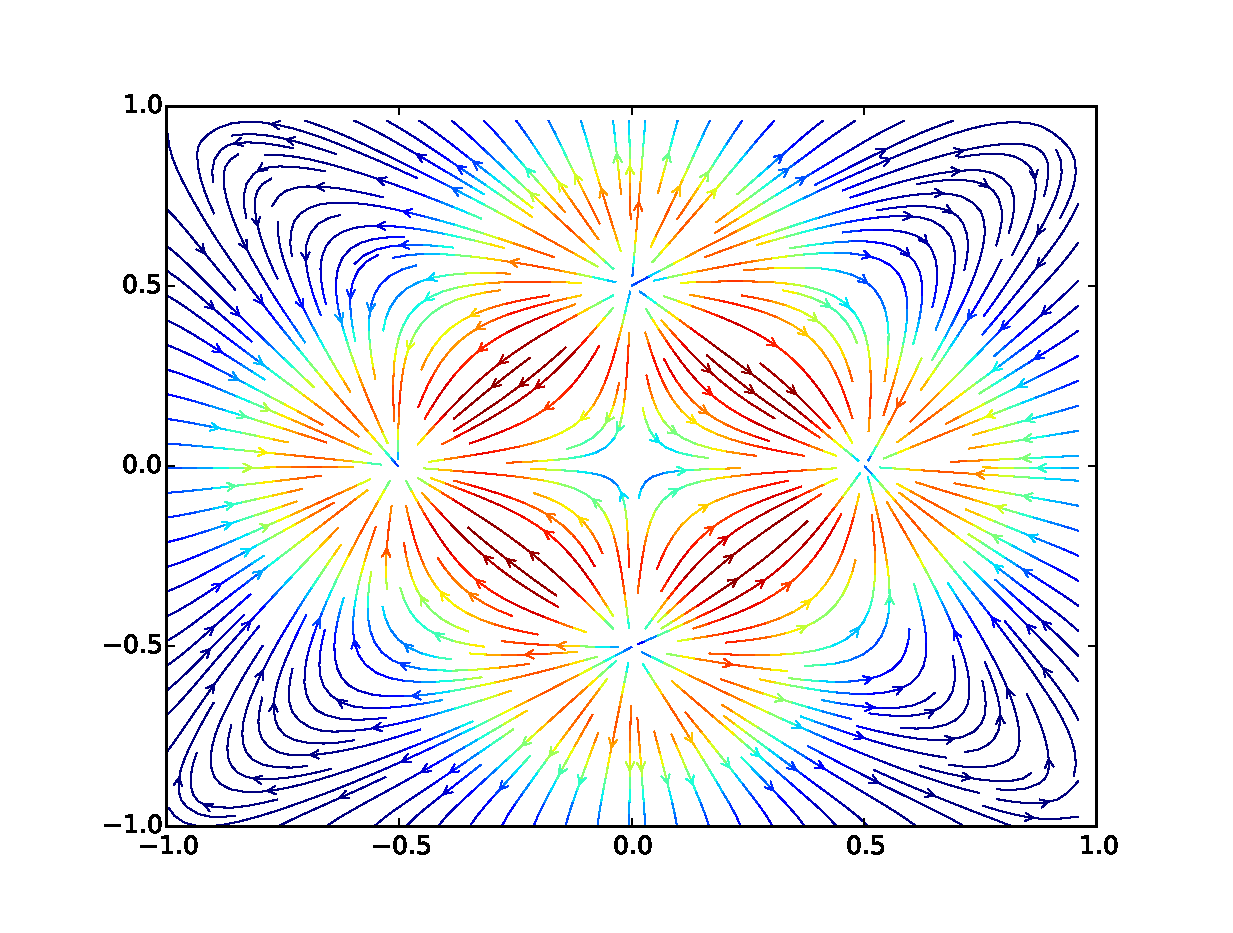
\includegraphics[trim=1.8cm 1cm 2cm 1cm,width=\textwidth,clip=true]{./gfx/curl_field.eps}
    \caption{Synthetic $2D$ curl-free field \label{fig:curl-field}.}
\end{figure}
\begin{figure}
    \centering
    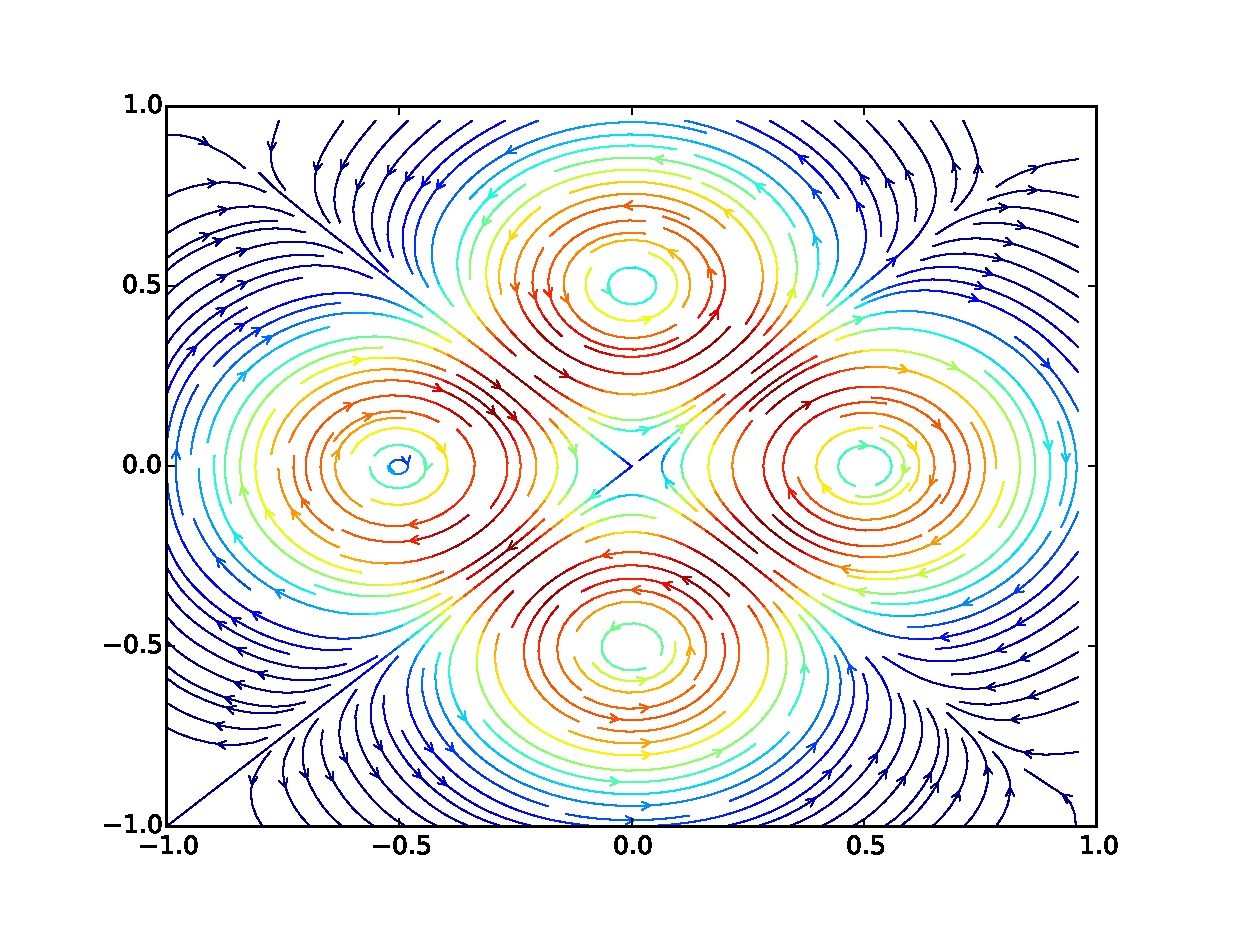
\includegraphics[trim=1.8cm 1cm 2cm 1cm,width=\textwidth,clip=true]{./gfx/div_field.eps}
    \caption{Synthetic $2D$ divergence-free field \label{fig:div-field}.}
\end{figure}
\begin{definition}[Curl-free and Div-free kernel \citep{Macedo2008}]
    \label{curl-div-free}
    Assume $\mathcal{X}=(\mathbb{R}^d, +)$ and $\mathcal{Y}=\mathbb{R}^p$ with
    $d=p$. The \emph{divergence-free} kernel is defined as
    \begin{dmath*}\label{div-def}
        K^{div}(x,z)=K^{div}_0(\delta) \hiderel{=} (\nabla\nabla^\transpose  -
        \Delta I) k_0(\delta)
    \end{dmath*}
    and the \emph{curl-free} kernel as
    \begin{dmath*}
        \label{curl-def} K^{curl}(x,z) \hiderel{=} K_0^{curl}(\delta)
        =-\nabla\nabla^\transpose k_0(\delta),
    \end{dmath*}
    where $\nabla$ is the gradient operator\mpar{See
    \cref{subsec:gradient_methods} for a formal definition of the operator
    $\nabla$.}, $\nabla\nabla^\transpose $ is the Hessian operator and $\Delta$
    is the Laplacian operator.
\end{definition}
Although taken separately these kernels are not universal, a convex combination
of the curl-free and divergence-free kernels allows to learn any vector field
that satisfies the Helmholtz decomposition theorem~\citep{Macedo2008,
Baldassare2012}. The next class of kernel we present are transformable kernels,
whose action on each coordinate of an outputs vector is determined by a
\say{views} of an input data.
\begin{definition}[Transformable kernel\citep{caponnetto2008}]
    Let $k:\mathcal{X}'\times\mathcal{X}'\to\mathbb{R}$ be a scalar-valued
    kernels and $\psi_1, \dots, \psi_p$ be a collection functions from
    $\mathcal{X}\to\mathcal{X}'$. Then the transformable kernel is defined for
    all $(i, j)\in(\mathbb{N}^*_p)^2$ as
    \begin{dmath*}
        K(x,z)_{ij} = \inner{e_i, K(x, z)e_j}_{\mathcal{Y}} \hiderel{=}
        k(\psi_i(x), \psi_j(z)),
    \end{dmath*}
    for all $x$, $z\in\mathcal{X}$.
\end{definition}
Transformable kernels have successfully used for network inference from time
series by means of autoregressive models (\citet{lim2013okvar,
lim2015operator}), and by \citet{vazquez2003multi} for cokriging the
multi-output version of kriging\mpar{Gaussian process regression.}, which takes
into account the correlations between the outputs.
\paragraph{}
We also introduce an example of \acl{OVK} acting on a function space which
found applications in \citet{kadri2015operator}.
\begin{definition}[Hilbert Schmidt Integral kernel \citep{kadri2015operator}]
    Let $k_{\mathcal{X}}:\mathcal{X}\times\mathcal{X}\to\mathbb{R}$ be a scalar
    valued kernel acting on the inputs and
    $k_{\mathcal{T}}:\mathcal{T}\times\mathcal{T} \to \mathbb{R}$ be a scalar
    valued kernel acting on the outputs. Define the integral operator
    $L_{\mathcal{T}} g = \int_{\mathcal{Y}}k_{\mathcal{T}}(\cdot,
    t)g(t)d\mu(t)$. Then the Hilbert Schmidt Integral kernel is defined as
    \begin{dmath*}
        K:
        \begin{cases}
            \mathcal{X}\times\mathcal{X} &\to \mathcal{L}(\mathcal{Y}) \\
            (x, z) &\mapsto k_{\mathcal{X}}(x, z) L_{\mathcal{T}}.
        \end{cases}
    \end{dmath*}
\end{definition}
This kernel is useful to learn functions $f$ that are function valued. In other
words, $f\in\mathcal{F}(\mathcal{X}; \mathcal{F}(\mathcal{T}; \mathbb{R}))$ and
the \acl{OVK} $K$ act on a function $g$ in the following way.
\begin{dmath}
    K(x, z)g = k_{\mathcal{X}}(x, z)\int_{\mathcal{Y}}k_{\mathcal{Y}}(\cdot,
    t)g(t)d\mu(t).
\end{dmath}
In \citet{kadri2015operator}, the author studied the case where
$\mathcal{T}=\mathbb{R}$ with $k_{\mathcal{Y}}(t, s)=\exp(-\abs{t-s})$ and
applied it to speech inversion (Which and how Human articulators are activated
from an audible speech signal). Notice that the Hilbert Schmidt integral kernel
is a particular case of decomposable kernel where
$\mathcal{Y}=\mathcal{F}(\mathcal{T}; \mathbb{R})$.

\chapterend
